% Rental-implied depreciation of AI accelerators. Built by `make paper`.
% Draft prose by Claude Code for AJ to rewrite (Decision 17). Every number is a macro from
% numbers.tex (gel.viz.paper_numbers) or a generated table; nothing is typed by hand.
\documentclass[11pt]{article}
\usepackage[margin=1in]{geometry}
\usepackage[T1]{fontenc}
\usepackage{lmodern}
\usepackage{microtype}
\usepackage{amsmath,amssymb}
\usepackage{booktabs}
\usepackage{graphicx}
\usepackage{caption}
\usepackage{xcolor}
\usepackage{adjustbox}
\usepackage[authoryear,round]{natbib}
\usepackage[hidelinks]{hyperref}
\usepackage{setspace}
\onehalfspacing

% Interpretations Claude drafted that AJ must confirm. \ajfinaltrue hides the marks.
\newif\ifajfinal
\ajfinalfalse
\ifdefined\ajfinalflag\ajfinaltrue\fi
\newcommand{\ajcheck}[1]{\ifajfinal#1\else{\color{blue!60!black}#1}\textsuperscript{\color{red}[AJ]}\fi}

% Generated by gel.viz.paper_numbers from paper/tables. Do not edit.
\newcommand{\nAcctFourFortyOiBnHi}{2.6}
\newcommand{\nAcctFourFortyOiBnLo}{$-$4.2}
\newcommand{\nAcctFourFortyOiPctHi}{3.3\%}
\newcommand{\nAcctFourFortyOiPctLo}{$-$11.0\%}
\newcommand{\nAcctFourFortyWorstEps}{$-$0.68}
\newcommand{\nAcctFourFortyWorstFirm}{Oracle}
\newcommand{\nAcctFourFortyWorstFy}{2026}
\newcommand{\nAcctFourFortyWorstPct}{$-$11.0\%}
\newcommand{\nAcctMsftCapexBn}{115.9}
\newcommand{\nAcctMsftFy}{2026}
\newcommand{\nAcctMsftGpuCapexBn}{34.8}
\newcommand{\nAcctRealOiBnHi}{12.4}
\newcommand{\nAcctRealOiBnLo}{1.5}
\newcommand{\nAcctRealOiPctHi}{15.5\%}
\newcommand{\nAcctRealOiPctLo}{2.6\%}
\newcommand{\nAcctSlFourOiBnHi}{1.5}
\newcommand{\nAcctSlFourOiBnLo}{$-$4.5}
\newcommand{\nAcctSlFourOiPctHi}{1.9\%}
\newcommand{\nAcctSlFourOiPctLo}{$-$10.4\%}
\newcommand{\nAwsSpotUnchanged}{17\%}
\newcommand{\nAwsVHundredFirstYear}{2017}
\newcommand{\nAwsVHundredLastYear}{2026}
\newcommand{\nAwsVHundredPrice}{3.06}
\newcommand{\nCovCrchipHi}{76\%}
\newcommand{\nCovCrchipLo}{74\%}
\newcommand{\nCovWcrHi}{98\%}
\newcommand{\nCovWcrLo}{98\%}
\newcommand{\nCovWcuHi}{72\%}
\newcommand{\nCovWcuLo}{66\%}
\newcommand{\nEvSixEleven}{$-$0.18}
\newcommand{\nFourShape}{0.47}
\newcommand{\nFourShapeHi}{0.57}
\newcommand{\nFourShapeLo}{0.36}
\newcommand{\nFourShapeOnDemand}{$-$0.13}
\newcommand{\nFourShapeOnDemandHi}{0.13}
\newcommand{\nFourShapeOnDemandLo}{$-$0.40}
\newcommand{\nFourShapePcm}{0.29}
\newcommand{\nFourShapeSpot}{0.87}
\newcommand{\nFourShapeSpotHi}{1.41}
\newcommand{\nFourShapeSpotLo}{0.34}
\newcommand{\nFourShapeWcrHi}{1.03}
\newcommand{\nFourShapeWcrLo}{$-$0.44}
\newcommand{\nFourShapeWcrP}{0.29}
\newcommand{\nFourShapeWcuP}{$<$0.0001}
\newcommand{\nGoogleShare}{62\%}
\newcommand{\nHHundredDispersion}{3.52}
\newcommand{\nHHundredHypNeo}{3.10}
\newcommand{\nHTwo}{$-$0.09}
\newcommand{\nHTwoHi}{0.23}
\newcommand{\nHTwoLo}{$-$0.40}
\newcommand{\nHyperscalerShare}{94\%}
\newcommand{\nListMoversRows}{5{,}226}
\newcommand{\nListTransitions}{9{,}282}
\newcommand{\nListUnchanged}{96\%}
\newcommand{\nMarkupShare}{47\%}
\newcommand{\nMcReps}{200}
\newcommand{\nNeocloudRows}{1{,}538}
\newcommand{\nOneARateEarly}{0.27}
\newcommand{\nOneARateEarlyHi}{0.77}
\newcommand{\nOneARateEarlyLo}{$-$0.23}
\newcommand{\nOneARateEarlyNoHTwoHundred}{$-$0.11}
\newcommand{\nOneARateLate}{$-$0.03}
\newcommand{\nOneARateLateHi}{0.18}
\newcommand{\nOneARateLateLo}{$-$0.24}
\newcommand{\nOneAShape}{0.31}
\newcommand{\nOneAShapeHi}{1.11}
\newcommand{\nOneAShapeLo}{$-$0.52}
\newcommand{\nOneBRateEarly}{0.28}
\newcommand{\nOneBRateEarlyHi}{0.84}
\newcommand{\nOneBRateEarlyLo}{$-$0.28}
\newcommand{\nOneBRateLate}{0.00}
\newcommand{\nOneBRateLateHi}{0.47}
\newcommand{\nOneBRateLateLo}{$-$0.50}
\newcommand{\nOneBShape}{0.28}
\newcommand{\nOneBShapeHi}{0.97}
\newcommand{\nOneBShapeLo}{$-$0.42}
\newcommand{\nPOneDHHundred}{$-$0.02}
\newcommand{\nPThreeAbundant}{11.0}
\newcommand{\nPThreeMedian}{4.1}
\newcommand{\nPThreeNoScarcity}{10.7}
\newcommand{\nPThreePNinety}{7.0}
\newcommand{\nPThreePTen}{2.2}
\newcommand{\nPTwoLopexHi}{11.7}
\newcommand{\nPTwoLopexLo}{9.8}
\newcommand{\nPanelRows}{24{,}210}
\newcommand{\nPathAHundredFive}{$-$0.45}
\newcommand{\nPathAHundredFivePct}{36\%}
\newcommand{\nPathHHundredFour}{$-$0.04}
\newcommand{\nPathHHundredFourPct}{4\%}
\newcommand{\nPathHHundredOne}{0.24}
\newcommand{\nPathHHundredOnePct}{$-$27\%}
\newcommand{\nPathHHundredThree}{$-$0.50}
\newcommand{\nPathHHundredThreePct}{40\%}
\newcommand{\nPathVHundredFour}{$-$0.13}
\newcommand{\nPathVHundredFourPct}{12\%}
\newcommand{\nPathVHundredNine}{$-$0.38}
\newcommand{\nPathVHundredNinePct}{32\%}
\newcommand{\nPermAssignments}{1{,}260}
\newcommand{\nPermP}{0.0008}
\newcommand{\nPermSharePositive}{55\%}
\newcommand{\nRawRows}{61{,}873}
\newcommand{\nSampleRows}{20{,}185}
\newcommand{\nShapeChipTrendZero}{$-$0.39}
\newcommand{\nShapeEqualProv}{0.19}
\newcommand{\nShapeListMovers}{$-$0.52}
\newcommand{\nShapeListMoversSe}{0.24}
\newcommand{\nShapeNoGoogle}{0.44}
\newcommand{\nTflopsCoef}{0.88}
\newcommand{\nTstarAll}{never}
\newcommand{\nTwoRateEarly}{0.11}
\newcommand{\nTwoRateEarlyHi}{0.35}
\newcommand{\nTwoRateEarlyLo}{$-$0.12}
\newcommand{\nTwoRateLate}{$-$0.15}
\newcommand{\nTwoRateLateHi}{0.11}
\newcommand{\nTwoRateLateLo}{$-$0.41}
\newcommand{\nTwoShape}{0.26}
\newcommand{\nTwoShapeHi}{0.47}
\newcommand{\nTwoShapeLo}{0.05}
\newcommand{\nTwoShapeWcrP}{0.30}
\newcommand{\nValFourFortyLostOne}{27\%}
\newcommand{\nValFourFortyLostThree}{72\%}
\newcommand{\nValFourFortyRentZero}{16.02}
\newcommand{\nValFourFortySle}{4.9}
\newcommand{\nValFourFortyVzeroCapex}{8.9}
\newcommand{\nValFourTwentyLostOne}{15\%}
\newcommand{\nValFourTwentyLostThree}{53\%}
\newcommand{\nValFourTwentyRentZero}{6.96}
\newcommand{\nValFourTwentySle}{7.1}
\newcommand{\nValFourTwentyVzeroCapex}{5.9}
\newcommand{\nValOpex}{0.30}
\newcommand{\nValRealLostOne}{11\%}
\newcommand{\nValRealLostThree}{32\%}
\newcommand{\nValRealRentZero}{5.85}
\newcommand{\nValRealSle}{9.4}
\newcommand{\nValRealSleFive}{5.1}
\newcommand{\nValRealSleSix}{6.1}
\newcommand{\nValRealVzeroCapex}{4.5}
\newcommand{\nValRealVzeroHi}{6.3}
\newcommand{\nValRealVzeroLo}{2.9}
\newcommand{\nValRentNow}{4.50}
\newcommand{\nValTwoLostOne}{6\%}
\newcommand{\nValTwoLostThree}{28\%}
\newcommand{\nValTwoRentZero}{4.83}
\newcommand{\nValTwoSle}{10.1}
\newcommand{\nValTwoVzeroCapex}{4.6}


\graphicspath{{figures/}}

\title{Rental-Implied Depreciation of AI Accelerators:\\ Why the Estimates Disagree}
\author{Ajai Upadhyaya\thanks{Virginia Commonwealth University. Working paper draft;
comments welcome. Replication package: see the data and code availability statement. Use of AI
tools: the code, data collection, analysis, figures and drafts of this paper were produced with
Claude (Anthropic), running in Claude Code, under the author's direction; see
Appendix~\ref{app:statements}.}}
\date{Draft, \today}

\begin{document}
\maketitle

\begin{abstract}
How fast do AI accelerators lose value? Published estimates range from roughly flat to about 40\% a
year. This paper rebuilds the question from posted rental prices: a panel of \nPanelRows{}
listing-months of NVIDIA V100 to B200 rents from October 2017 to November 2026, across hyperscalers
and neoclouds and across on-demand, spot and reserved contracts. Because age equals calendar time
minus vintage, the age profile is not identified with chip and month effects, so the paper
reports each chip's realized price path and four identification strategies side by side. Three
findings stand out. First, realized rents fall slowly: the V100's rent changes by \nPathVHundredNine{}
log points over nine years. Second, the shape of the age profile depends on
the market read: spot prices fall late, while list prices that actually change fall early, and
\nListUnchanged{} of month-to-month on-demand and reserved transitions show no change at all.
Third, with valid few-cluster inference no strategy identifies a significant decline or shape.
Turning rents into asset values, rents stay far above power and maintenance costs for the whole
observed life, so economic life is set by obsolescence and power scarcity rather than by rents
reaching operating cost. \ajcheck{The disagreement in the literature is largely a disagreement
about which price series and which identification assumption to use.}

\end{abstract}

\section{Introduction}
\label{sec:intro}

Reported earnings at the largest AI spenders now hinge on one management estimate: how many years
a server lasts. Between 2020 and 2025 Microsoft, Alphabet, Amazon, Meta, Oracle and CoreWeave
lengthened the useful lives of their servers, and Amazon partly reversed course for a subset of
them in 2025 (Section~\ref{sec:background} and Table~\ref{tab:lives}). Whether five- or six-year
straight-line lives are defensible for graphics processing units (GPUs) bought at the peak of an
investment boom is now a live question for investors, auditors and regulators.

The first academic and practitioner estimates of accelerator depreciation have appeared, and they
disagree. \citet{amissahocran2026collateral} fit a rent--age profile at one date and find a
retention path consistent with roughly 40\% a year; \citet{chincholikar2026economic} use executed
resale prices and find 24--27\%; \citet{huang2026gpu} measure rental contribution on a
peer-to-peer marketplace and find 17--32\%; and archived posted on-demand prices show declines
from roughly 15\% a year to none at all \citep{ccir2026rental}. These studies measure different
things: resale value, net cash flow or posted rent, at one date or along a path.

This paper puts those measurements on one basis, using the object that is easiest to observe
over time: what it costs to rent an accelerator for an hour. I build a panel of \nPanelRows{}
listing-months of posted rents for seven NVIDIA chips, from the V100 (2017) to the B200 (2024),
covering October 2017 to November 2026. It combines Amazon Web Services (AWS) price-list history,
archived pricing pages, the SkyPilot catalog history and live collection, across hyperscalers and
neoclouds and across on-demand, spot and reserved contracts (Section~\ref{sec:data}).

The central econometric problem is old. Age equals calendar time minus vintage, so with chip and
month fixed effects the linear part of the age profile is not identified \citep{hall1968technical}.
Following the advice to report each chip's realized path first, I then run four identification
strategies side by side: a quality-adjusted vintage effect, a frontier-relative obsolescence term
after \citet{geske2007computers}, a successor event study, and a shape-only specification that
sweeps an assumed linear rate (Section~\ref{sec:method}). Inference is at the chip level, which
leaves seven clusters.

Three results stand out.

\emph{Realized rents fall slowly.} Holding provider, region and contract fixed, the V100's rent
changes by \nPathVHundredFour{} log points over its first four years and \nPathVHundredNine{}
over nine; the A100 40GB's falls to \nPathAHundredFive{} by year five. The H100's rent rose by
\nPathHHundredOne{} in its first year and was \nPathHHundredThree{} at three years, before 2026's
shortage brought it back to \nPathHHundredFour{} at four years.

\emph{The shape of the age profile depends on the market, and the data mostly measure pricing
habits.} \nListUnchanged{} of month-to-month on-demand and reserved transitions in the panel show
no price change; AWS has charged \$\nAwsVHundredPrice{} an hour for a V100 on demand in every year
from \nAwsVHundredFirstYear{} to \nAwsVHundredLastYear{}. Spot prices give a back-loaded profile
(rate over years 0--2 minus the rate over years 2--4 of \nFourShapeSpot), while list prices that
do change give a front-loaded one (\nShapeListMovers, provider-clustered standard error
\nShapeListMoversSe). \ajcheck{Which of these is ``the'' age profile is a choice of market, not a
technical detail.}

\emph{With valid inference, the data do not pin down the rate or the shape.} Under the
unrestricted wild cluster bootstrap that the analysis pre-registered, the pooled shape estimate
(\nFourShape) excludes zero. A Monte Carlo on this panel's design shows that the unrestricted
bootstrap's 95\% intervals cover the truth only \nCovWcuLo--\nCovWcuHi{} of the time, while the
restricted version covers about \nCovWcrHi; under the restricted bootstrap the shape has
$p = \nFourShapeWcrP$ and a 95\% interval of [\nFourShapeWcrLo, \nFourShapeWcrHi]. No
identification strategy that identifies a linear rate finds a significant decline over years 0--4.

Turning rents into asset values (Section~\ref{sec:values}), the present value of net rent falls
along the realized path by \nValRealLostThree{} by year three for an H100, which is slower than any
five- or six-year straight-line schedule. The H100's neocloud rent of \$\nValRentNow{} an hour
compares with roughly \$\nValOpex{} of power and maintenance, so rents never fall to operating cost within the
nine-year horizon: economic life is set by obsolescence and power scarcity, not by rents reaching
operating cost. A separate benchmark, term-structure and retirement analysis
(Section~\ref{sec:triangulation}) places the power-constrained retirement age at
\nPThreeMedian{} years and the life to operating cost at \nPTwoLopexLo--\nPTwoLopexHi{} years,
with book lives in between.

\ajcheck{The contribution is a reconciliation. The spread of published rates comes mostly from
three choices that are rarely stated: which price series is read (resale, spot, posted list, or
transacted rent), which identification assumption pins the linear age term, and whether value is
taken to end when rent reaches operating cost or when a better chip displaces the old one in a
power-constrained slot.} The paper's open panel, code and identification range let readers make
those choices explicitly.

\paragraph{Related literature.} The paper applies the vintage-price approach to depreciation
\citep{hulten1981estimation, oliner1993constant, doms2004computers, geske2007computers} and
hedonic price measurement \citep{rosen1974hedonic, berndt1993price, triplett2006handbook} to a new
asset class with an active rental market, as \citet{gavazza2011leasing} does for aircraft. Its
identification problem is the age--period--cohort problem of \citet{hall1968technical} and
\citet{deaton1997analysis}. On inference with few clusters it follows
\citet{cameron2008bootstrap}, \citet{mackinnon2017wild}, \citet{webb2023reworking} and
\citet{mackinnon2023cluster}. On the accounting side it relates to \citet{keating1999depreciation}.
Recent work measures cloud prices \citep{byrne2018cloud, sawyer2023ppi} and GPU price-performance
\citep{hobbhahn2022trends}, and a fast-growing practitioner and working-paper literature argues
about accelerator lives \citep{dutta2026priced, rosenzweig2026second}.

\section{Institutional background}
\label{sec:background}

\subsection{Useful lives in financial statements}

Under U.S. GAAP a firm depreciates property and equipment over its estimated useful life, and a
change in that estimate is applied prospectively as a change in accounting estimate. Servers and
network equipment are reported inside property and equipment, and no firm in the sample reports
GPUs as a separate asset class. Table~\ref{tab:lives} lists the server useful-life policies and
changes disclosed by the seven firms studied here, each with the filing it comes from
(\texttt{docs/useful\_lives.md} holds the exact quotations and accession numbers).

\begin{table}[htbp]
\centering
\caption{Server useful-life policies and changes disclosed in SEC filings}
\label{tab:lives}
\begin{adjustbox}{max width=\textwidth}
\IfFileExists{tables/p7_useful_lives.tex}{% Generated by gel.viz.paper_numbers from config/accounting.yaml (book_life).
\begin{tabular}{lll}
\hline
Firm & Fiscal year of effect & Server useful life (years) \\
\hline
Microsoft & 2021 & 3 $\to$ 4 \\
Microsoft & 2023 & 4 $\to$ 6 \\
Alphabet & 2021 & 3 $\to$ 4 \\
Alphabet & 2023 & 4 $\to$ 6 \\
Amazon & 2020 & 3 $\to$ 4 \\
Amazon & 2022 & 4 $\to$ 5 \\
Amazon & 2024 & 5 $\to$ 6 \\
Amazon & 2025 & 6 $\to$ 5 \\
Meta & 2022 & 4 $\to$ 4.5 \\
Meta & 2023 & 4.5 $\to$ 5 \\
Meta & 2025 & 5 $\to$ 5.5 \\
Oracle & 2023 & 4 $\to$ 5 \\
Oracle & 2025 & 5 $\to$ 6 \\
CoreWeave & 2023 & 5 $\to$ 6 \\
Nebius & 2026 & 4 $\to$ 5 \\
\hline
\end{tabular}
}{\emph{Table generated in Phase 7.}}
\end{adjustbox}
\par\smallskip\footnotesize Source: 10-K and 20-F filings on SEC EDGAR; quotations and accession
numbers in the replication package.
\end{table}

The economic stakes are large because server capital expenditure has grown fast: a one-year
change in the assumed life of a cohort of servers moves annual depreciation by billions of dollars
at each of the largest spenders (Section~\ref{sec:accounting}).

\subsection{How accelerators are rented}

Accelerators are rented by the hour in three main ways. Hyperscalers (AWS, Microsoft Azure and
Google Cloud) post on-demand list prices for every region and instance type, discounted prices for
one- and three-year commitments, and interruptible spot prices. Neoclouds (here Lambda, CoreWeave
and Paperspace) post simpler price lists, often per GPU-hour. Marketplaces match owners and
renters at transacted prices but restrict automated collection, so they are not collected here.
Large customers negotiate private prices that are not posted anywhere; this paper is therefore
about the posted-price market, and Section~\ref{sec:robust} discusses what that implies.

\ajcheck{Posted prices differ in how often they move. Hyperscaler on-demand and reserved list prices
are revised rarely and in large steps, while spot prices respond to spare capacity. The age profile
one reads depends on which of these series is used, which is the theme of
Section~\ref{sec:profiles}.}

\section{Data}
\label{sec:data}

\subsection{Sources}

The panel combines four kinds of source, each archived as raw files with the source URL,
retrieval time and HTTP status. (1) AWS's public price-list offer files, which give on-demand and
reserved list prices roughly monthly since 2015. (2) The SkyPilot project's public catalog history,
which records AWS, Azure, Google Cloud and Lambda list and spot prices since mid-2022. SkyPilot's
catalog carries no licence, so it is used but not redistributed. (3) Archived pricing pages for
Lambda, CoreWeave and Paperspace from the Internet Archive's Wayback Machine. (4) Live daily
collection from October 2026 (the Azure Retail Prices API, AWS offer files, Lambda's pricing page
and SkyPilot). Chip specifications and release dates come from Epoch AI's hardware database
\citep{epoch2026hardware}, electricity prices from the U.S. Energy Information Administration,
and the deflator is the BLS CPI-U \citep{blscpiu}. Vast.ai, RunPod and Oracle restrict automated
collection, so nothing is collected from them.

\subsection{Construction}

The unit of observation is one posted price for a provider, SKU, chip, GPU count, interconnect,
region, contract type and term in one month, in U.S. dollars per GPU-hour; multi-GPU instance
prices are divided by the GPU count. From \nRawRows{} raw rows, zone-level spot prices become one
regional median per day, daily observations become one monthly median, and where two collectors
record the same offer in the same month the more direct source is kept (the two agree to a median
gap of zero). The result is \nPanelRows{} listing-months from October 2017 to November 2026. Real
prices are in 2025 dollars. The estimation sample drops the L40S (no release date), the MI300X (one
month), outlier-flagged prices and the partial month of November 2026, leaving \nSampleRows{}
listing-months for seven NVIDIA chips (Table~\ref{tab:sample}).

\begin{table}[htbp]
\centering
\caption{Estimation sample by chip}
\label{tab:sample}
\begin{adjustbox}{max width=\textwidth}
% Generated by gel.viz.paper_numbers from p4_descriptive_facts.csv and p5_sample.csv.
\begin{tabular}{lrrrrrr}
\hline
Chip & Listing-months & Providers & First month & Ages (months) & Hyperscaler/neocloud & Max/min provider \\
\hline
V100 & 5{,}260 & 6 & 2017-10 & 3--111 & 1.61 & 3.10 \\
A100 40GB & 5{,}510 & 6 & 2020-11 & 6--77 & 2.34 & 2.67 \\
A100 80GB & 3{,}081 & 6 & 2022-05 & 18--71 & 1.92 & 2.47 \\
H100 PCIe & 355 & 3 & 2023-01 & 4--49 & 2.66 & 1.95 \\
H100 SXM & 4{,}831 & 6 & 2023-01 & 4--49 & 3.10 & 3.52 \\
H200 & 664 & 4 & 2024-12 & 1--23 & 0.73 & 1.73 \\
B200 & 484 & 4 & 2025-06 & 7--23 & 1.54 & 2.08 \\
\hline
\end{tabular}

\end{adjustbox}
\par\smallskip\footnotesize Listing-months in the estimation sample; ages in months since the
Epoch release month. ``Hyperscaler/neocloud'' is the median ratio of median on-demand prices in
months where both provider types list the chip; ``Max/min provider'' is the median ratio of the
most to the least expensive provider's median on-demand price.
\end{table}

\subsection{What the raw panel shows}

The panel is mostly hyperscaler list prices: hyperscalers account for \nHyperscalerShare{} of
listing-months and Google Cloud alone for \nGoogleShare{} of the estimation sample, because it
publishes every region and machine shape. Neocloud history (\nNeocloudRows{} listing-months)
comes from archived pages. Three features of the raw data matter for everything that follows.

\emph{Prices barely move.} \nListUnchanged{} of the \nListTransitions{} month-to-month transitions
in on-demand and reserved listings show no price change; AWS spot prices, by contrast, are
unchanged in only \nAwsSpotUnchanged{} of transitions.

\emph{Levels differ widely across providers.} For the H100 SXM the median hyperscaler on-demand
price is \nHHundredHypNeo{} times the neocloud price, and the most expensive provider's median is
\nHHundredDispersion{} times the cheapest's in a typical month (Table~\ref{tab:sample},
Figure~\ref{fig:prices}).

\emph{Raw prices rise with age for the newest chips} (Figure~\ref{fig:prices}, right), because age
moves one-for-one with calendar time, with the 2023--26 shortages and with which providers list a
chip. \ajcheck{None of this is an age effect, which is why the paper does not read age profiles off
raw prices.}

\begin{figure}[htbp]
\centering
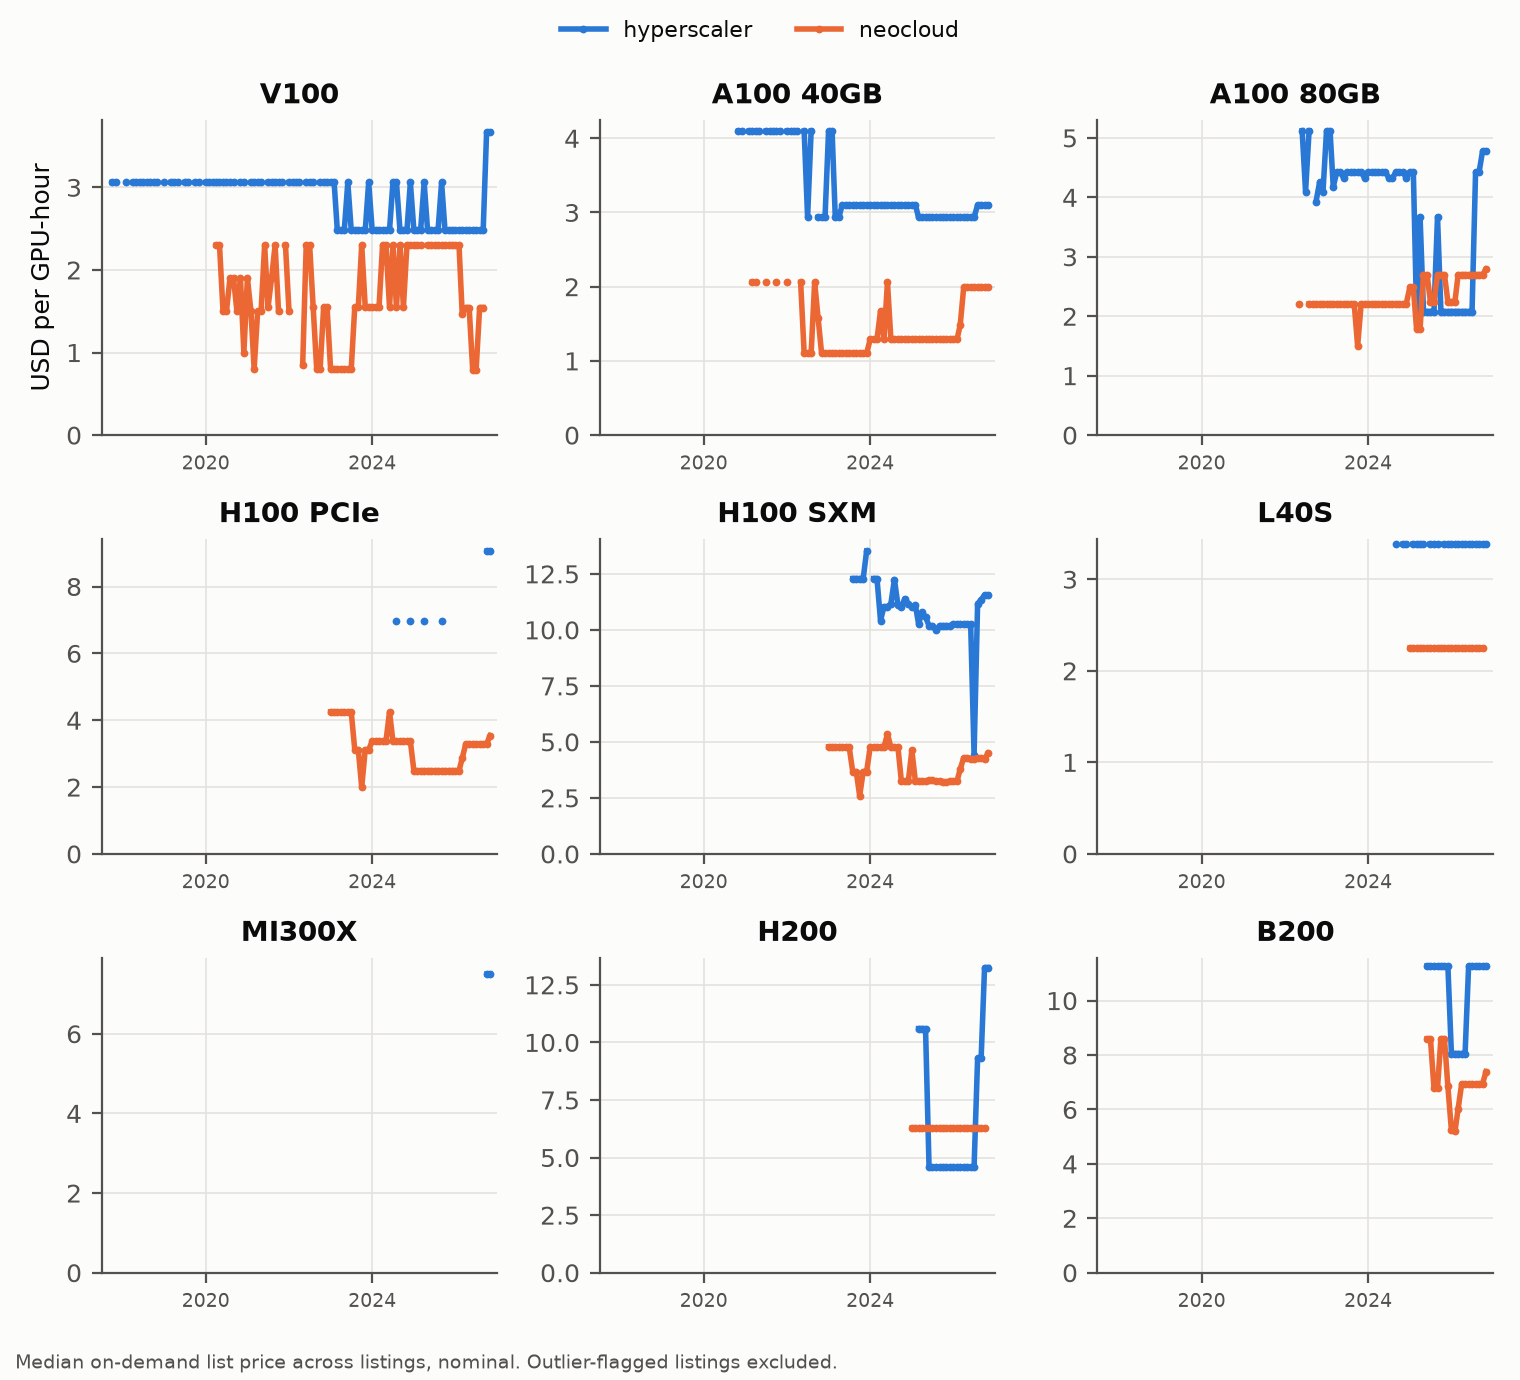
\includegraphics[width=0.49\textwidth]{p4a_price_by_chip.png}
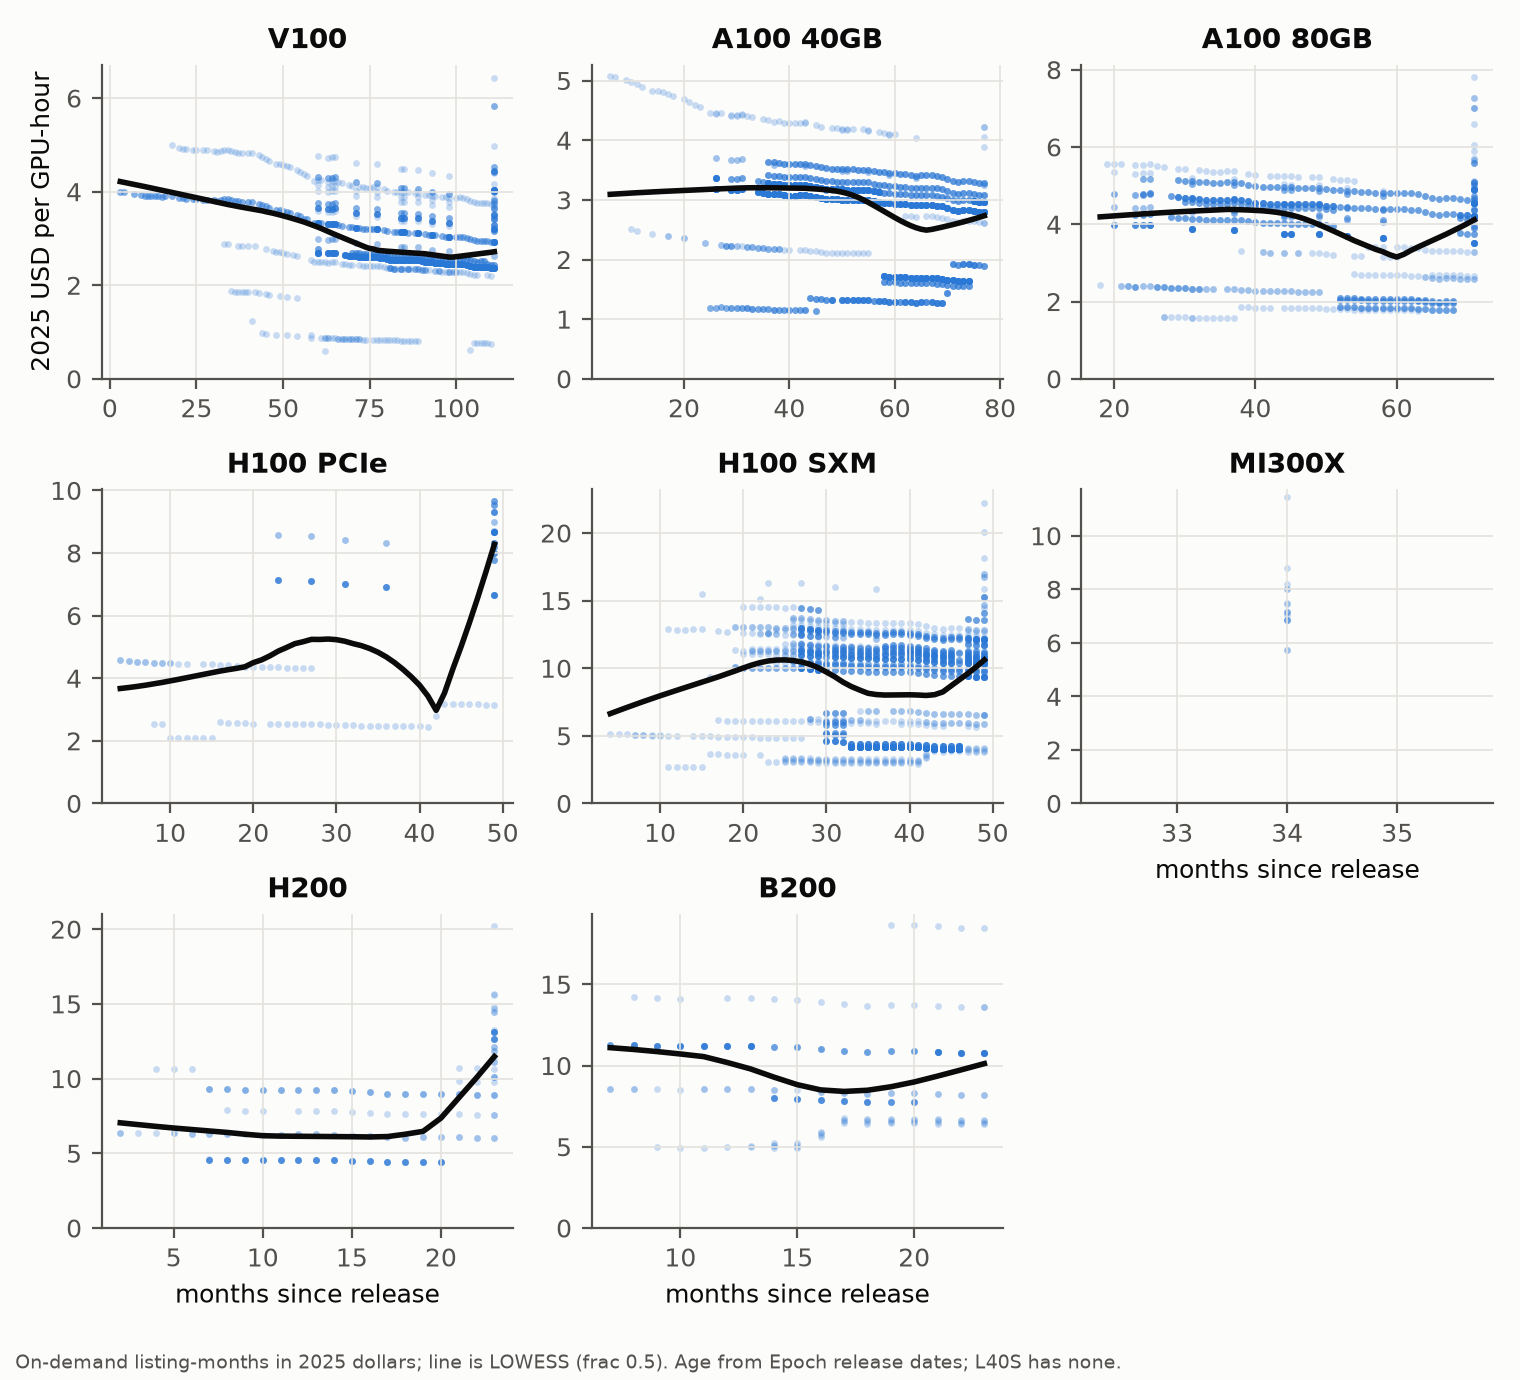
\includegraphics[width=0.49\textwidth]{p4b_price_vs_age.png}
\caption{On-demand prices by chip over time (left) and real prices against age (right). Source:
the panel described in Section~\ref{sec:data}; outlier-flagged listings excluded.}
\label{fig:prices}
\end{figure}

\section{Methodology}
\label{sec:method}

\subsection{Hedonic rental-price model}

For listing $i$ of chip $c$ in month $t$,
\begin{equation}
\ln p_{ict} = \alpha_c + g(a_{ct}) + \delta_t + X_i'\beta + \varepsilon_{ict},
\label{eq:hedonic}
\end{equation}
where $p$ is the real posted price per GPU-hour, $a_{ct}$ the chip's age in years since its release
month, $g$ the age profile, $\alpha_c$ a chip (vintage) effect, $\delta_t$ a month effect and $X_i$
fixed effects for provider $\times$ region, contract type $\times$ term, GPUs per instance, price
basis (instance or accelerator only) and form factor. $g$ is a cubic spline in age with knots at
1.5, 3 and 5 years. The specifications were logged before any regression was run, together with
four hypotheses. H1, front-loaded decline: value falls fastest in a chip's first two years, closer
to geometric than to straight-line. H2, obsolescence shocks: a successor's release causes a
discrete drop in the predecessor's rent. H3, contract-type wedge: spot and on-demand prices fall
faster with age than reserved prices. H4, demand regimes: shortages mask age effects only
temporarily, so age profiles are stable across sub-periods once month effects are included.

\subsection{Identification}

Because $a_{ct} = t - v_c$, any linear trend in age can be moved into the chip and month effects,
so the linear part of $g$ is not identified in \eqref{eq:hedonic} \citep{hall1968technical}. Its
curvature is identified, but only through differences in calendar-time trends across vintages:
$a^2 = t^2 - 2 v t + v^2$, and $-2vt$ is a chip-specific trend. I report five objects.

\begin{enumerate}
\item \emph{Observed cohort paths.} Each chip's price path, by six-month age bin, with the controls
but without month effects. This needs no identification assumption: it is what happened.
\item \emph{Strategy 1, quality-adjusted vintage.} Replace $\alpha_c$ with observed specifications:
(a) $\ln$ BF16 dense TFLOP/s alone, and (b) adding $\ln$ memory bandwidth and $\ln$ memory. The
linear age term is then identified from the cross-chip relation between residual price and release
date.
\item \emph{Strategy 2, frontier-relative obsolescence.} Keep $\alpha_c$, drop $\delta_t$ and add the
chip's TFLOP/s relative to the best chip released by month $t$, after \citet{geske2007computers}.
The assumption is that market-wide time effects work only through the frontier.
\item \emph{Strategy 3, successor event study.} Event-time dummies around the release of each
chip's successor (V100 at A100, A100 at H100, H100 at B200), with chip and month effects.
\item \emph{Strategy 4, shape only.} Keep both sets of effects, identify only the curvature, and
report $g_d(a) = d\,a + \tilde c(a)$ over a grid of assumed average rates $d$ from 0 to $-0.40$
log points a year, where $\tilde c$ is the curvature detrended over ages 0--6.
\end{enumerate}

The summary measures are $g(1)-g(0)$, $g(2)-g(0)$, $g(4)-g(0)$, the average annual log change over
years 0--2 and 2--4, and their difference, the \emph{early minus late rate}. H1 predicts a negative
early minus late rate. Strategy 4 reports only that
difference, the one measure that does not depend on the assumed linear term.

\subsection{Inference}

Age has one value per chip and month, so inference is at the chip level, with seven clusters. The
method specified in advance is the unrestricted wild cluster bootstrap with Webb's six-point weights and
9,999 draws \citep{cameron2008bootstrap, webb2023reworking}. Cluster-robust standard errors by
provider and two-way by provider and month are shown for comparison. After the adversarial review
(Appendix~\ref{app:review}) I add the restricted bootstrap (WCR), which imposes the null when generating draws and is
recommended when clusters are few and unequal in size \citep{mackinnon2017wild,
mackinnon2023cluster}, a test-inversion interval, and a Monte Carlo of interval coverage on this
panel's design.

\subsection{From rents to asset values}

The value of a chip at age $a$ is the present value of its remaining net rent,
\begin{equation}
V(a) = \sum_{m = 0}^{12(H - a) - 1} \frac{730 \, \max\{u\,p(a + m/12) - o,\ 0\} \, S(m)}{(1+r)^{(m+1)/12}},
\label{eq:value}
\end{equation}
summed over remaining months $m$ at 730 hours a month, with utilization $u$, operating cost per GPU-hour $o$ (system
power $\times$ PUE $\times$ electricity price, plus maintenance at 4\% of capital cost a year),
survival $S$ at a 2\% annual failure rate, discount rate $r$ and horizon $H$ of nine years, the
oldest age observed. The rent path is $p(a) = p_{\text{now}} \exp\{g(a) - g(a_{\text{now}})\}$:
each chip's current neocloud median on-demand rent moved along a profile $g$ from the realized
cohort paths or one of the strategies. I report $V(0)$ relative to capital cost, the share of value
lost by each year, the economic life $T^*$ (the first age at which $u p \le o$), and a
straight-line-equivalent life $L = 2\int_0^H V(a)/V(0)\,da$, the straight-line life with the same
average book value. The base case is $r = 10\%$, $u = 70\%$ and a PUE of 1.3; the grid is
$r \in \{8, 10, 12\}\%$, $u \in \{50, 70, 90\}\%$ and PUE $\in \{1.2, 1.4\}$.

\subsection{Earnings restatement}

Section~\ref{sec:accounting} enters each year's estimated GPU capital expenditure as a purchase
cohort and depreciates it under the firm's disclosed straight-line life and under the
rental-implied schedules from \eqref{eq:value}, with the GPU share of capital expenditure varied
over a grid because no firm discloses it.

\section{Results}
\label{sec:results}

\subsection{Observed price paths}
\label{sec:paths}

Figure~\ref{fig:paths} shows each chip's realized price path relative to its first observed
six-month bin, holding provider, region, contract and the other controls fixed. These paths need
no identification assumption. The older chips decline slowly and unevenly: the V100 changes by
\nPathVHundredFour{} log points over four years and \nPathVHundredNine{} over nine, and the A100
40GB reaches \nPathAHundredFive{} at five years. The H100's rent instead rose in its first year
(\nPathHHundredOne), fell to \nPathHHundredThree{} at three years, and recovered to
\nPathHHundredFour{} at four years in the 2026 shortage. \ajcheck{Realized paths are not smooth
decays. They are long flat stretches, sharp falls and demand-driven rebounds, and the 2026 shortage
reverses part of the decline for every chip still on sale.}

\begin{figure}[htbp]
\centering
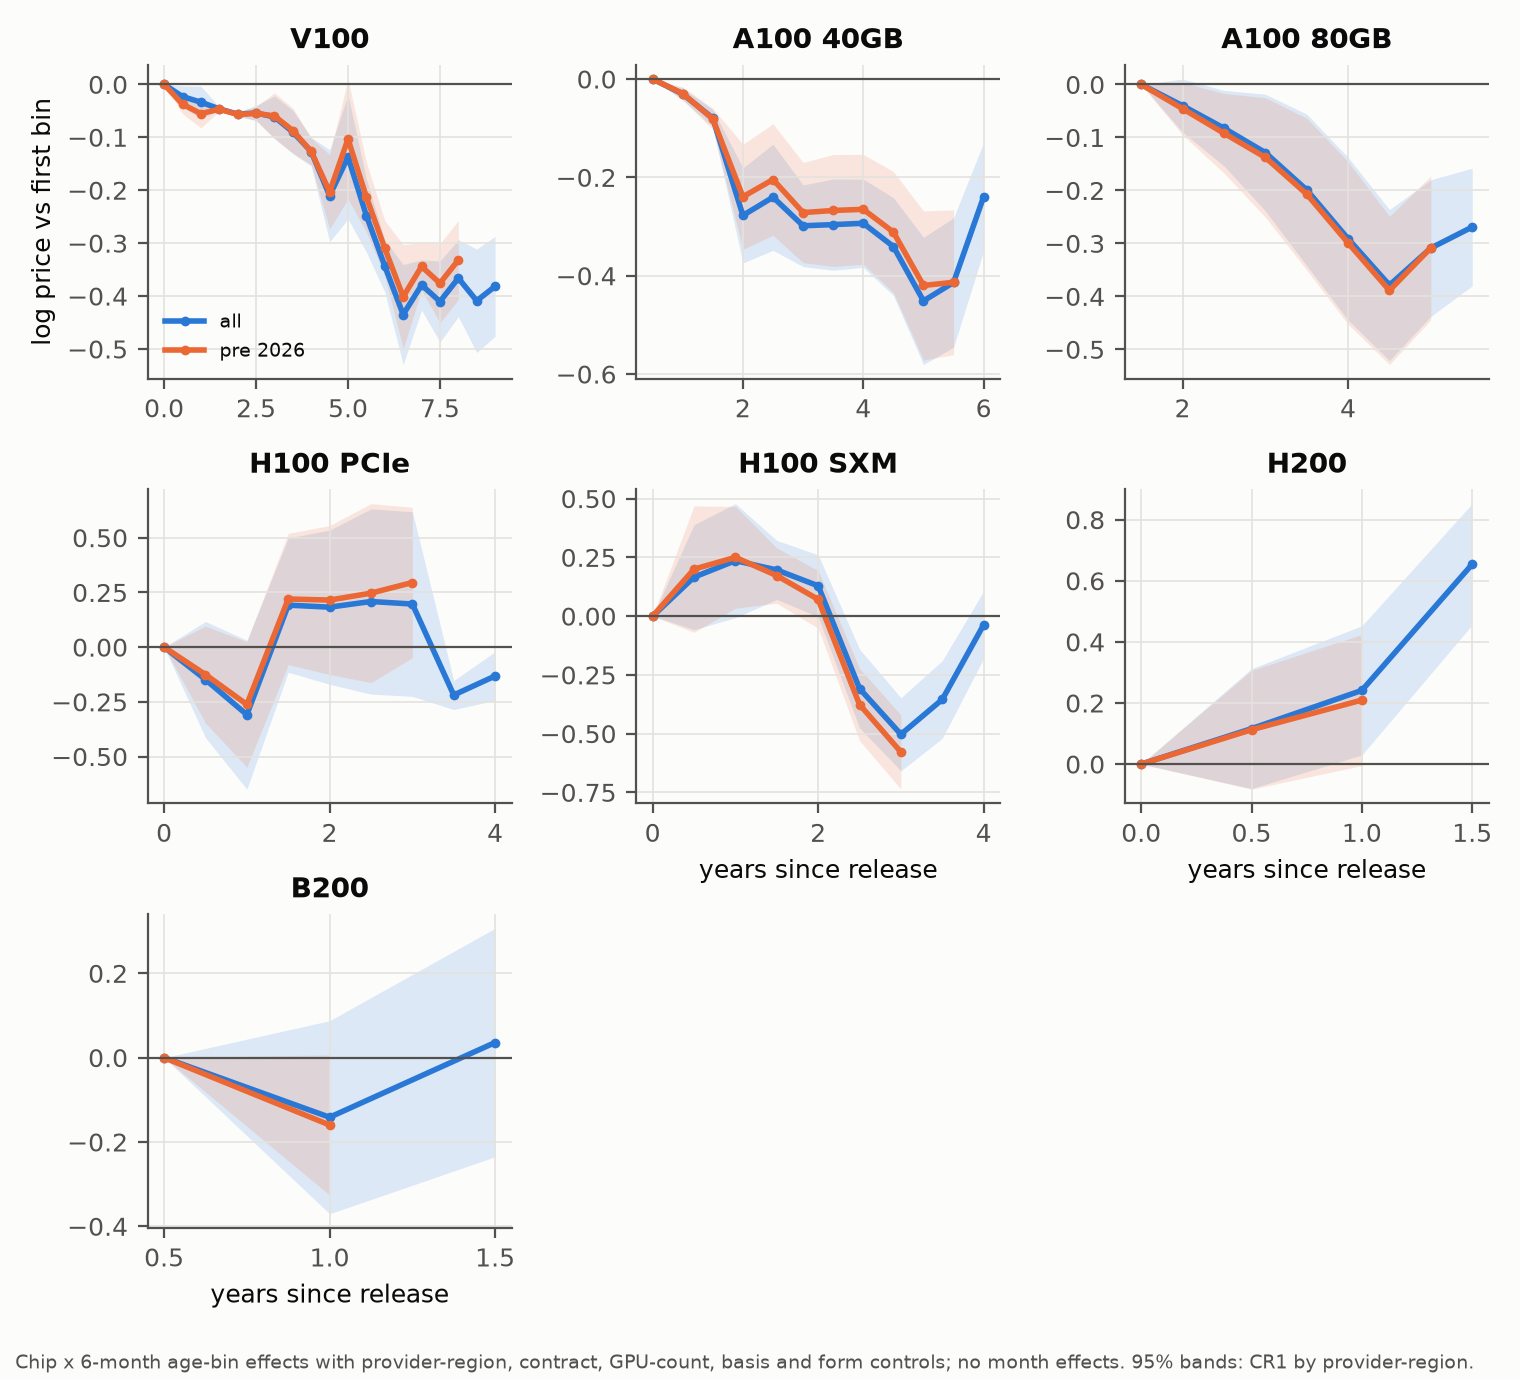
\includegraphics[width=0.85\textwidth]{p5a_cohort_paths.png}
\caption{Observed cohort paths: log real price by six-month age bin relative to each chip's first
bin, with provider $\times$ region, contract $\times$ term, GPU count, price basis and form-factor
controls and no month effects. Bands: 95\% intervals, CR1 by provider-region.}
\label{fig:paths}
\end{figure}

\subsection{Age profiles under four identification strategies}
\label{sec:profiles}

Table~\ref{tab:strategies} and Figure~\ref{fig:profiles} report the strategies that identify a
linear term, and the shape-only strategy. Strategy 1 prices each log point of TFLOP/s at
\nTflopsCoef{} log points of rent. It finds no decline with age over the first two years (rate
\nOneARateEarly, interval [\nOneARateEarlyLo, \nOneARateEarlyHi]) and roughly none after
(\nOneARateLate). Strategy 2's age profile rises slightly and then falls (\nTwoRateEarly{} and
\nTwoRateLate{} a year). Strategy 4's shape estimate is \nFourShape{}
[\nFourShapeLo, \nFourShapeHi] under the pre-registered bootstrap. Every point estimate of the
early minus late rate is positive: prices fall later, not earlier, against H1.

\begin{table}[htbp]
\centering
\caption{Summary of the age profile by identification strategy (full sample)}
\label{tab:strategies}
\begin{adjustbox}{max width=\textwidth}
% Generated by gel.viz.hedonic_figures from p5_summary.csv. Do not edit.
\begin{tabular}{lccccc}
\hline
Strategy & $g(2)-g(0)$ & $g(4)-g(0)$ & rate, yrs 0--2 & rate, yrs 2--4 & early $-$ late rate (H1: $<0$) \\
\hline
1a quality index (TFLOP/s) & 0.55 [-0.45, 1.55] & 0.48 [-0.06, 1.03] & 0.27 [-0.23, 0.77] & -0.03 [-0.24, 0.18] & 0.31 [-0.52, 1.11] \\
1b three specs & 0.55 [-0.57, 1.68] & 0.55 [-0.61, 1.69] & 0.28 [-0.28, 0.84] & -0.00 [-0.50, 0.47] & 0.28 [-0.42, 0.97] \\
2 frontier-relative & 0.22 [-0.25, 0.69] & -0.08 [-0.77, 0.62] & 0.11 [-0.12, 0.35] & -0.15 [-0.41, 0.11] & 0.26 [0.05, 0.47] \\
4 shape only & -- & -- & -- & -- & 0.47 [0.36, 0.57] \\
\hline
\end{tabular}

\end{adjustbox}
\par\smallskip\footnotesize Log points; rates are per year. Brackets: 95\% intervals from the
unrestricted wild cluster bootstrap at the chip level (7 clusters, Webb weights, 9,999 draws). These
intervals are too narrow; see Table~\ref{tab:review}.
\end{table}

\begin{figure}[htbp]
\centering
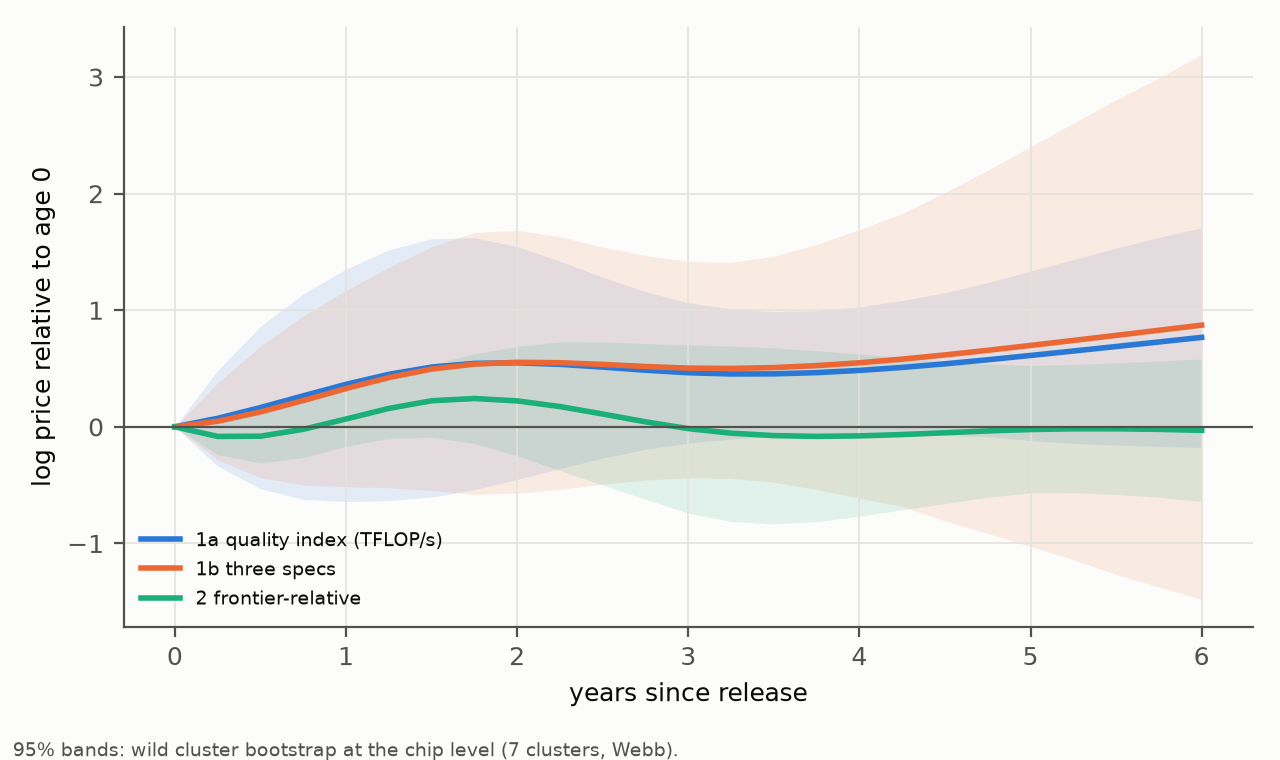
\includegraphics[width=0.49\textwidth]{p5b_strategy_profiles.png}
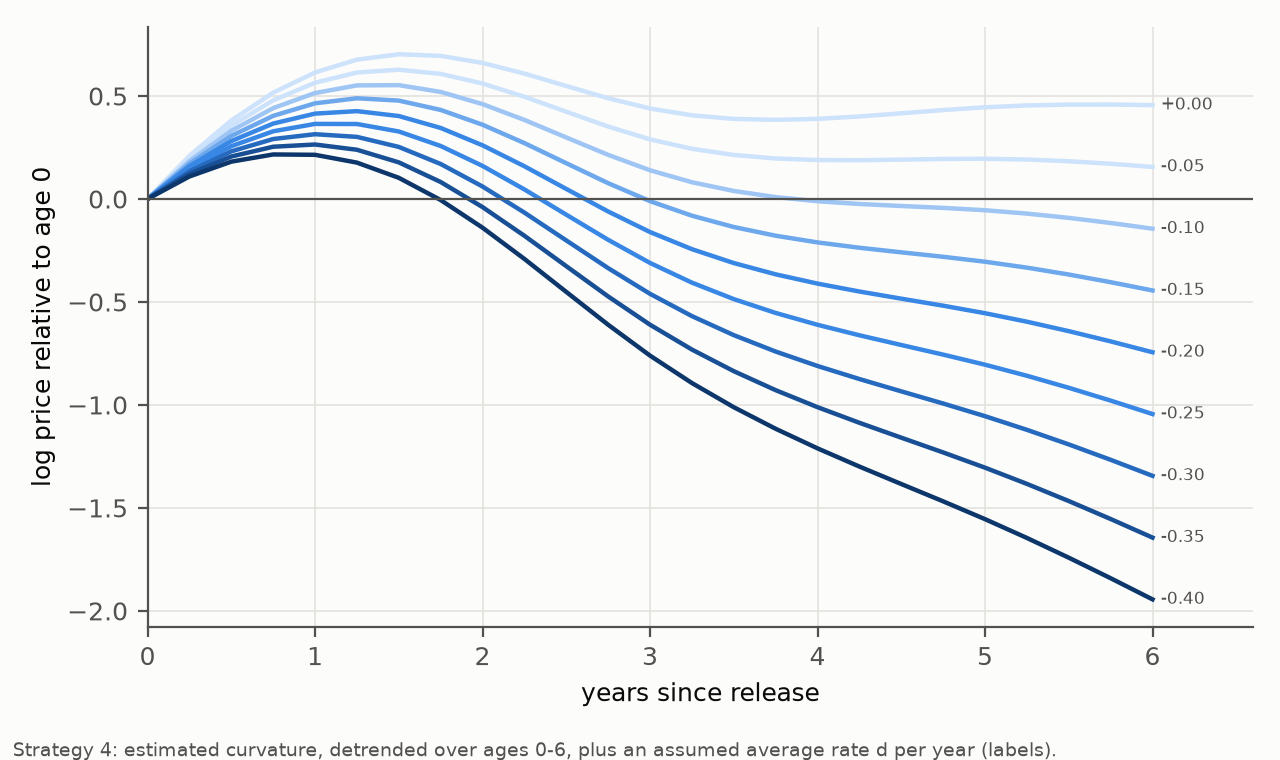
\includegraphics[width=0.49\textwidth]{p5c_strategy4_sweep.png}
\caption{Age profiles $g(a) - g(0)$ under strategies 1a, 1b and 2 (left) and strategy 4 for
assumed average rates $d$ from 0 to $-0.40$ log points a year (right).}
\label{fig:profiles}
\end{figure}

\subsection{What survives valid inference}
\label{sec:review}

An adversarial review of these results, written by a reader with no access to the author's notes,
identified three problems; Table~\ref{tab:review} and the checks below address them.

\emph{The intervals are too narrow.} In a Monte Carlo that keeps this panel's rows, fixed effects
and regressors and draws errors with the estimated residual structure under a true shape of zero,
the unrestricted bootstrap's 95\% intervals cover the truth \nCovWcuLo--\nCovWcuHi{} of the time
and CR1 by chip \nCovCrchipLo--\nCovCrchipHi{} (\nMcReps{} replications per design); the restricted
bootstrap covers \nCovWcrLo--\nCovWcrHi. Under the restricted bootstrap no summary measure is
significant: strategy 4's shape has $p = \nFourShapeWcrP$ (unrestricted $p$ \nFourShapeWcuP) and
a test-inversion interval of [\nFourShapeWcrLo, \nFourShapeWcrHi], and strategy 2's has
$p = \nTwoShapeWcrP$.

\emph{The shape is identified only from vintage-specific trends.} Allowing each chip its own
linear calendar trend leaves the quadratic term unidentified; at a zero quadratic term the shape is
\nShapeChipTrendZero. Reassigning release dates across chips, the actual assignment gives the
largest shape of \nPermAssignments{} distinct assignments ($p = \nPermP$), so the curvature is tied
to release order. \ajcheck{That test cannot tell an age effect from demand trends that are
themselves ordered by vintage, such as the 2023--26 shortages that hit the newest chips.}

\emph{The answer depends on the market.} The shape is \nFourShapeSpot{} for spot prices
[\nFourShapeSpotLo, \nFourShapeSpotHi] and \nFourShapeOnDemand{} for on-demand prices
[\nFourShapeOnDemandLo, \nFourShapeOnDemandHi]. Restricting to the \nListMoversRows{} non-spot
listings whose price changes at least once, it is \nShapeListMovers{} (provider-clustered standard
error \nShapeListMoversSe), in H1's direction. Weighting providers equally cuts the pooled shape to
\nShapeEqualProv.

\begin{table}[htbp]
\centering
\caption{Unrestricted (WCU) and restricted (WCR) wild cluster bootstrap $p$-values}
\label{tab:review}
% Generated by gel.viz.paper_numbers from p5_review_wcr.csv.
\begin{tabular}{llrrrr}
\hline
Strategy & Measure & Estimate & SE (CR1, chip) & $p$ (WCU) & $p$ (WCR) \\
\hline
1a quality index & rate, yrs 0--2 & 0.27 & 0.16 & 0.300 & 0.649 \\
1a quality index & rate, yrs 2--4 & $-$0.03 & 0.06 & 0.615 & 0.678 \\
1a quality index & early $-$ late & 0.31 & 0.19 & 0.421 & 0.735 \\
1b three specs & rate, yrs 0--2 & 0.28 & 0.16 & 0.262 & 0.595 \\
1b three specs & rate, yrs 2--4 & 0.00 & 0.14 & 0.991 & 0.993 \\
1b three specs & early $-$ late & 0.28 & 0.22 & 0.591 & 0.820 \\
2 frontier-relative & rate, yrs 0--2 & 0.11 & 0.09 & 0.297 & 0.494 \\
2 frontier-relative & rate, yrs 2--4 & $-$0.15 & 0.06 & 0.208 & 0.228 \\
2 frontier-relative & early $-$ late & 0.26 & 0.10 & 0.006 & 0.305 \\
4 shape only & early $-$ late & 0.47 & 0.08 & $<$0.0001 & 0.287 \\
\hline
\end{tabular}

\par\smallskip\footnotesize Null: measure $= 0$. Chip-level clusters (7), Webb weights, 9,999
draws. SE: CR1 clustered by chip.
\end{table}

\ajcheck{Taken together, the projection strategies do not establish either the speed or the shape
of the age profile in this sample. The observed cohort paths are the more credible guide to the
rate, and the dependence of the shape on the market read is itself a finding.}

\subsection{Successor releases}
\label{sec:events}

Figure~\ref{fig:events} shows the predecessor's price around its successor's release. There is no
detectable drop: prices in the first year after release are \nHTwo{} [\nHTwoLo, \nHTwoHi] relative
to the six months before. The one negative bin, \nEvSixEleven{} at 6--11 months, falls where cloud
availability of the successor actually began; dating events by the successor's first listing in
the panel moves that bin earlier, and neither dating detects a drop (H2).

\begin{figure}[htbp]
\centering
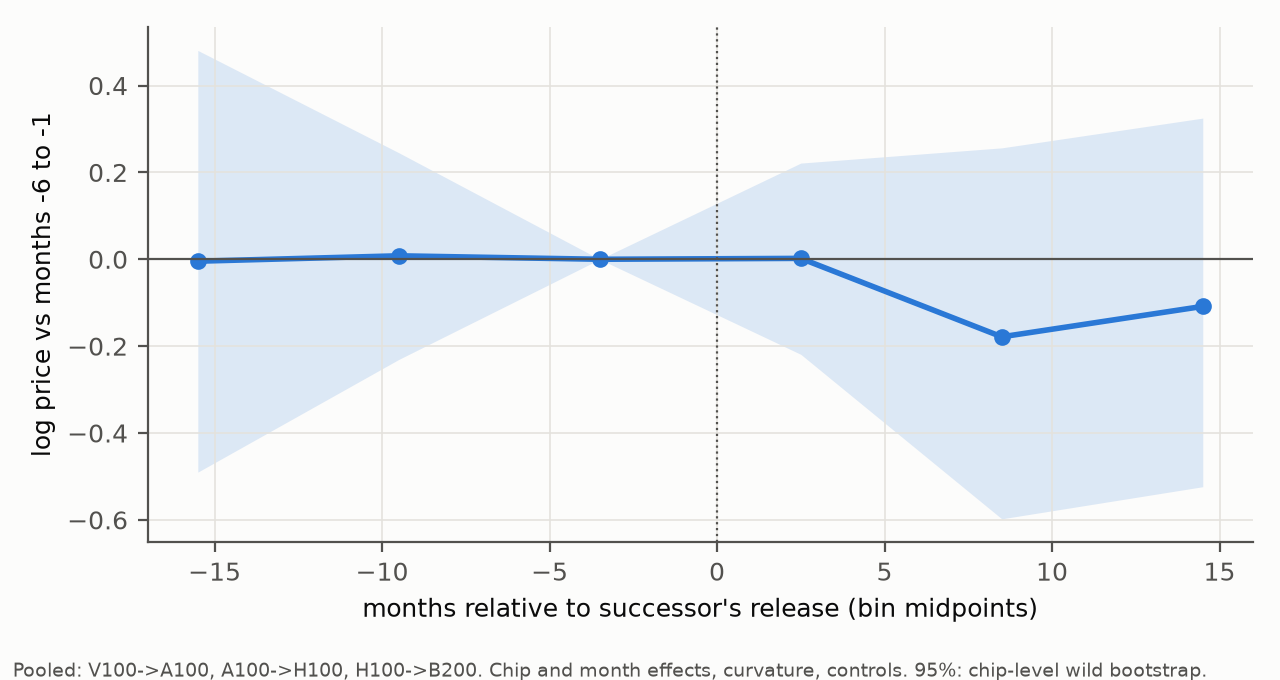
\includegraphics[width=0.6\textwidth]{p5d_event_study.png}
\caption{Successor event study: predecessor prices by six-month event-time bin around the
successor's Epoch release month, relative to months $-6$ to $-1$; chip and month effects and
controls. Bands: unrestricted chip-level bootstrap.}
\label{fig:events}
\end{figure}

\subsection{Asset values and economic life}
\label{sec:values}

Table~\ref{tab:values} and Figure~\ref{fig:values} turn the rent paths into values. Along the
realized path an H100 loses \nValRealLostOne{} of its value in the first year and
\nValRealLostThree{} by year three, and its straight-line-equivalent life is \nValRealSle{} years:
value declines more slowly than under any five- or six-year straight-line schedule. Strategy 2 gives
a similar curve (\nValTwoLostThree{} by year three). Only an assumed average decline of
0.40 log points a year in strategy 4 produces a front-loaded curve (\nValFourFortyLostThree{} lost by
year three, life \nValFourFortySle{} years), and it implies a launch rent of \$\nValFourFortyRentZero{}
an hour for the H100, far above any rent in the panel.

\begin{table}[htbp]
\centering
\caption{Asset values and straight-line-equivalent lives}
\label{tab:values}
\begin{adjustbox}{max width=\textwidth}
% Generated by gel.models.asset_value from p6_summary.csv. Do not edit.
% Base case r = 10%, u = 70%, PUE 1.3, system power, 2%/yr failure; brackets: min-max over the r x u x PUE grid.
\begin{tabular}{llcccc}
\hline
Chip & Rent path & $V(0)$/capex & Share lost by yr 3 & SL-equivalent life (yrs) & $T^*$ (yrs) \\
\hline
A100 80GB & Realized (V100, A100) & 5.32 [3.41, 7.48] & 0.32 [0.31, 0.33] & 9.4 [9.2, 9.6] & $>$9 \\
A100 80GB & 2 frontier-relative & 4.83 [3.07, 6.83] & 0.28 [0.27, 0.30] & 10.1 [9.8, 10.3] & $>$9 \\
A100 80GB & 4 shape, d = -0.20 & 9.08 [6.02, 12.48] & 0.52 [0.52, 0.53] & 7.2 [7.0, 7.3] & $>$9 \\
A100 80GB & 4 shape, d = -0.40 & 19.94 [13.58, 26.82] & 0.71 [0.71, 0.72] & 5.0 [4.9, 5.1] & $>$9 \\
H100 SXM & Realized (V100, A100) & 4.49 [2.89, 6.31] & 0.32 [0.31, 0.33] & 9.4 [9.2, 9.6] & $>$9 \\
H100 SXM & 2 frontier-relative & 4.55 [2.91, 6.41] & 0.28 [0.27, 0.30] & 10.1 [9.9, 10.3] & $>$9 \\
H100 SXM & 4 shape, d = -0.20 & 5.89 [3.87, 8.11] & 0.53 [0.52, 0.54] & 7.1 [6.9, 7.3] & $>$9 \\
H100 SXM & 4 shape, d = -0.40 & 8.89 [6.00, 12.02] & 0.72 [0.72, 0.74] & 4.9 [4.8, 5.0] & $>$9 \\
H200 & Realized (V100, A100) & 5.57 [3.60, 7.80] & 0.32 [0.31, 0.33] & 9.4 [9.2, 9.6] & $>$9 \\
H200 & 2 frontier-relative & 4.81 [3.08, 6.79] & 0.28 [0.27, 0.30] & 10.1 [9.9, 10.3] & $>$9 \\
H200 & 4 shape, d = -0.20 & 4.00 [2.58, 5.57] & 0.54 [0.53, 0.56] & 7.0 [6.7, 7.2] & $>$9 \\
H200 & 4 shape, d = -0.40 & 3.81 [2.49, 5.23] & 0.76 [0.74, 0.79] & 4.5 [4.1, 4.7] & $>$9 \\
B200 & Realized (V100, A100) & 4.45 [2.87, 6.23] & 0.32 [0.31, 0.33] & 9.4 [9.2, 9.6] & $>$9 \\
B200 & 2 frontier-relative & 3.84 [2.45, 5.42] & 0.28 [0.27, 0.30] & 10.1 [9.8, 10.3] & $>$9 \\
B200 & 4 shape, d = -0.20 & 3.18 [2.05, 4.44] & 0.54 [0.53, 0.57] & 7.0 [6.7, 7.1] & $>$9 \\
B200 & 4 shape, d = -0.40 & 3.03 [1.97, 4.17] & 0.76 [0.75, 0.80] & 4.4 [4.0, 4.7] & $>$9 \\
\hline
\end{tabular}

\end{adjustbox}
\par\smallskip\footnotesize $V(0)$/capex: value at release over capital cost. SL-equivalent life:
$2\int_0^H V(a)/V(0)\,da$. $T^*$: first age at which utilization $\times$ rent $\le$ operating cost.
Operating cost excludes hosting, network and staff, so $V(0)$/capex is an upper bound.
\end{table}

\begin{figure}[htbp]
\centering
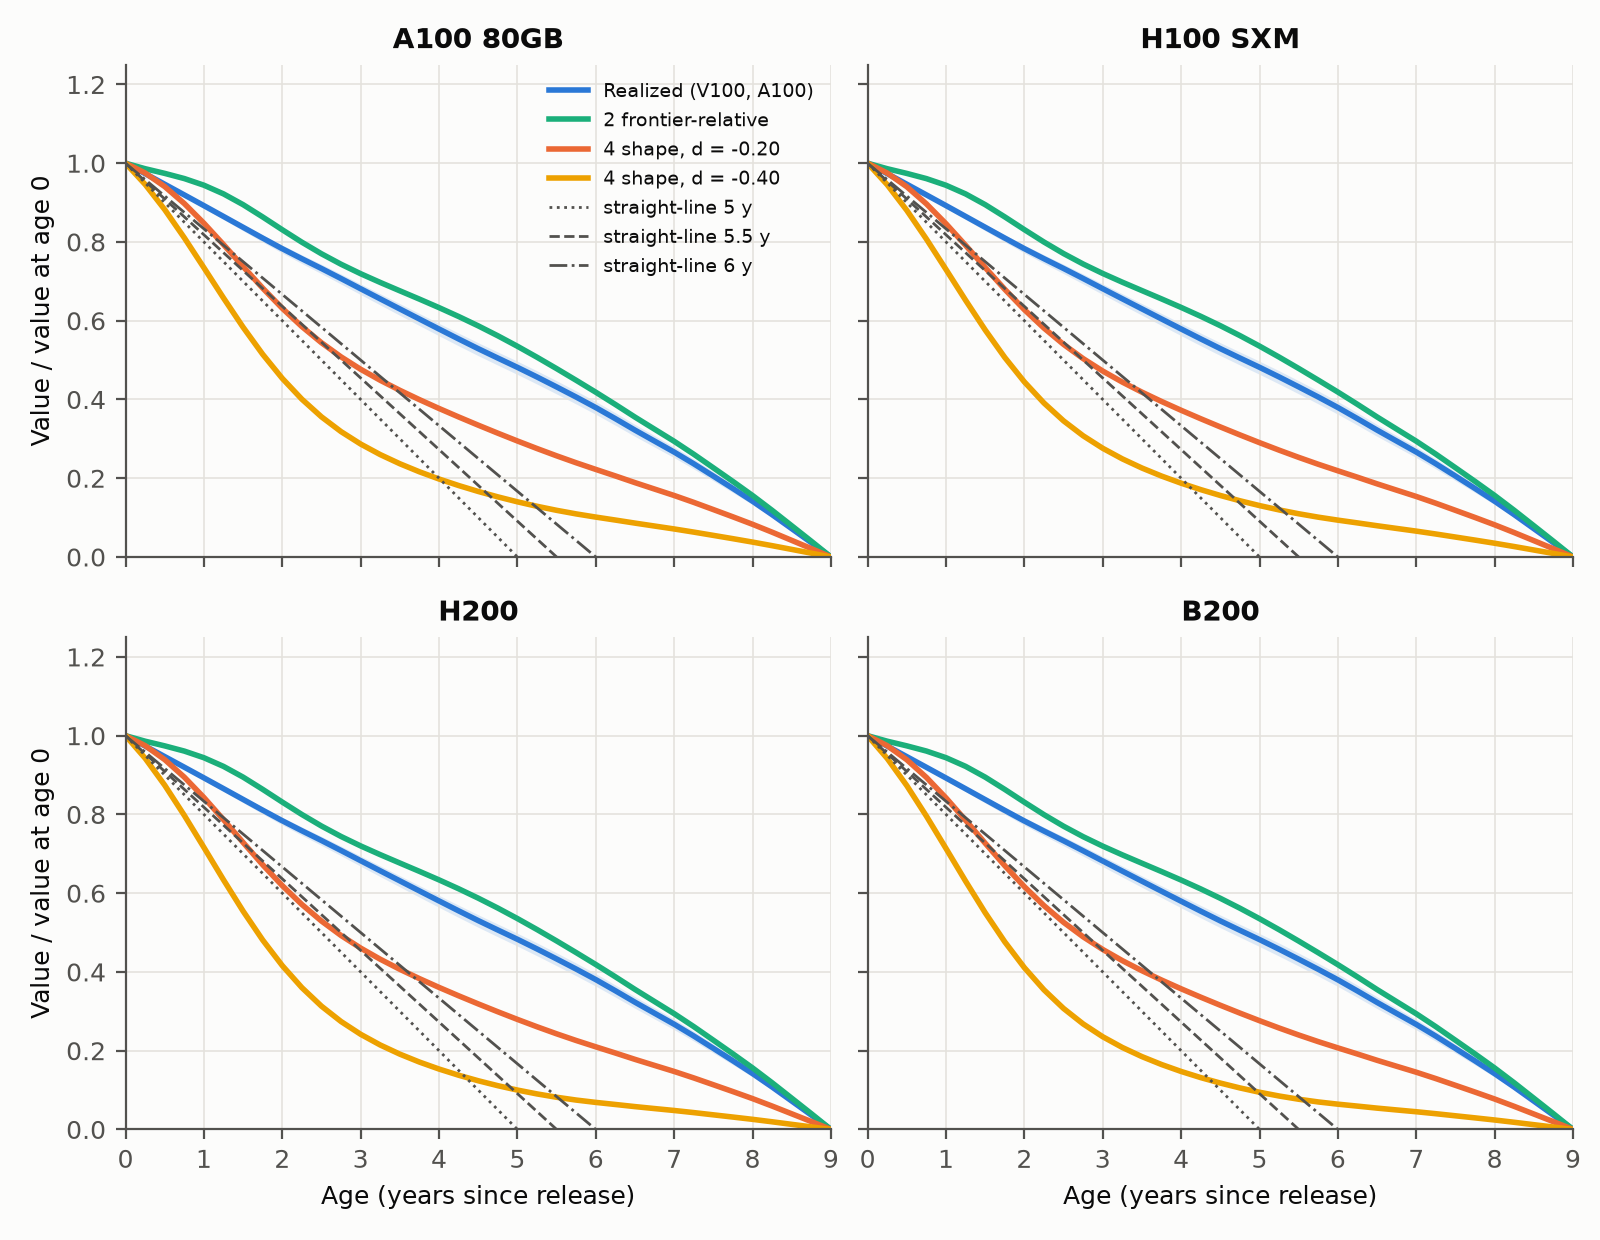
\includegraphics[width=0.85\textwidth]{p6_value_curves.png}
\caption{Value relative to value at release, by rent path, against 5-, 5.5- and 6-year
straight-line schedules. Band: the $r \times u \times$ PUE grid around the realized path.}
\label{fig:values}
\end{figure}

Two features of these numbers matter more than their levels. First, $T^*$ \nTstarAll{} binds within
the nine-year horizon: the H100's neocloud rent of \$\nValRentNow{} an hour is many times its
\$\nValOpex{} of power and maintenance, so the end of the value curve is set by the horizon, not by
rents reaching operating cost. With a six-year horizon the straight-line-equivalent life is
\nValRealSleSix{} years, and with five years \nValRealSleFive. \ajcheck{Rents alone do not pin down
economic life; the retirement decision does.} Second, $V(0)$ is \nValRealVzeroLo--\nValRealVzeroHi{}
times capital cost across the grid, which reflects scarcity rents and the omitted hosting costs, so
the value-to-cost ratio should not be read as profitability.

\subsection{Triangulation with benchmark, term-structure and retirement evidence}
\label{sec:triangulation}

A companion analysis measures three other quantities for the same chips: a throughput benchmark
priced at neocloud rents (P1), the decay implied by reserved-to-on-demand price ratios (P2), and a
power-constrained retirement model in which an old chip is replaced when a newer one would earn
more in the same power slot (P3). Table~\ref{tab:triangulation} and Figure~\ref{fig:triangulation}
compare them. Old chips are priced close to their output today (the H100's obsolescence discount
against the H200 is \nPOneDHHundred). Life to operating cost is long: \nPTwoLopexLo--\nPTwoLopexHi{}
years for the H100 from the term structure. In the power-constrained model the median retirement
age is \nPThreeMedian{} years (P10--P90 \nPThreePTen--\nPThreePNinety), rising to
\nPThreeAbundant{} years when power is abundant and \nPThreeNoScarcity{} without a scarcity markup;
about \nMarkupShare{} of today's rent is markup at the calibrated level. \ajcheck{Book lives of four
to six years sit between the power-constrained and the unconstrained answers, close to the
constrained one.}

\begin{table}[htbp]
\centering
\caption{Triangulation of economic life by method}
\label{tab:triangulation}
\begin{adjustbox}{max width=\textwidth}
% Generated by gel.viz.paper_numbers from m8_triangulation.csv.
\begin{tabular}{lrrrr}
\hline
Generation (age, yrs) & P1 discount $D$ & P1 life to opex & P2 life to opex & P3 retirement age (P10--P90) \\
\hline
A100 80GB (6.0) & 0.00 [$-$0.21, 0.20] & 19.9--25.9 & 10.7--13.2 & 4.1 (2.2--7.0) \\
H100 SXM (4.1) & $-$0.02 [$-$0.13, 0.34] & 15.1--20.4 & 9.8--11.7 & 4.1 (2.2--7.0) \\
H200 SXM (2.0) & 0.00 [0.00, 0.00] & 14.3--18.8 & 6.5--7.5 & 4.1 (2.2--7.0) \\
\hline
\end{tabular}

\end{adjustbox}
\par\smallskip\footnotesize P1: obsolescence discount against the H200 at concurrency 32 (median
neocloud price; provider range) and implied life to operating cost. P2: life to operating cost over
the discount-rate and term-premium grid. P3: median retirement age, power-constrained base case.
All lives in years since release.
\end{table}

\begin{figure}[htbp]
\centering
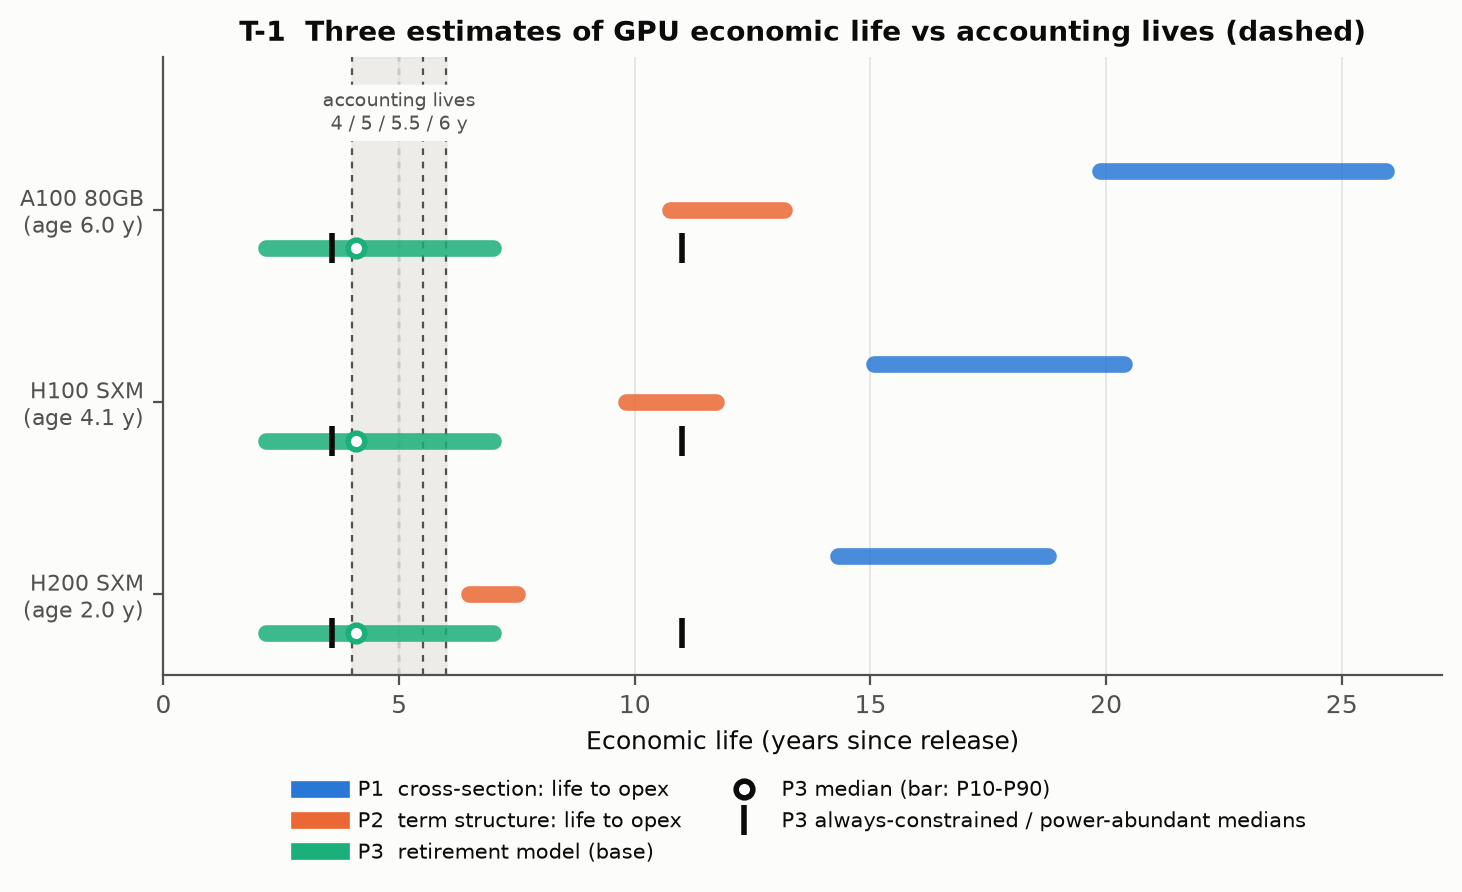
\includegraphics[width=0.75\textwidth]{t1_triangulation.png}
\caption{Economic life by method against accounting lives of 4, 5, 5.5 and 6 years.}
\label{fig:triangulation}
\end{figure}

\section{Accounting implications}
\label{sec:accounting}

\IfFileExists{sections/accounting_body.tex}{No firm reports GPUs separately, so the restatement estimates a GPU asset base. Each year's cash
capital expenditure from XBRL is multiplied by the share that is servers and network equipment
(0.6 in the baseline, 0.4 and 0.8 as alternatives; no firm discloses it) and by the GPU share of
server spending (0.3 to 0.8). For Microsoft in fiscal \nAcctMsftFy, for example, \$\nAcctMsftCapexBn{}
billion of capital expenditure becomes a GPU base of \$\nAcctMsftGpuCapexBn{} billion at a GPU share
of one half. Each year's purchases form a cohort from fiscal 2020, depreciated under the firm's
disclosed straight-line life (Table~\ref{tab:lives}; changes applied prospectively, as the firms
did) and under each alternative schedule. The change in operating income is the negative of the
change in depreciation; the change in diluted EPS applies the firm-year effective tax rate.
Every firm-year number traces to an XBRL fact listed with its accession number in the replication
package.

Table~\ref{tab:restate} reports the latest fiscal year for each firm. Under the rental-implied
schedule built on the realized cohort paths, which depreciates slower than any of the disclosed
lives, the five hyperscalers' operating income would be \nAcctRealOiPctLo--\nAcctRealOiPctHi{}
\emph{higher} (\$\nAcctRealOiBnLo--\nAcctRealOiBnHi{} billion) at a GPU share of one half. Under
the steepest schedule, strategy 4 with an assumed decline of 0.40 log points a year, the change
ranges from \nAcctFourFortyOiPctLo{} to \nAcctFourFortyOiPctHi{}; the largest cut is
\nAcctFourFortyWorstFirm's, \nAcctFourFortyWorstPct{} of fiscal \nAcctFourFortyWorstFy{} operating
income, or \$\nAcctFourFortyWorstEps{} per diluted share. A four-year straight-line life gives a
similar range (\nAcctSlFourOiPctLo{} to \nAcctSlFourOiPctHi). CoreWeave and Nebius, whose operating
income is small relative to their GPU spending, are shown in dollars only.

\begin{table}[htbp]
\centering
\caption{Change in operating income and diluted EPS under alternative GPU depreciation schedules,
latest fiscal year}
\label{tab:restate}
\begin{adjustbox}{max width=\textwidth}
% Generated by src/gel/accounting/restate.py from paper/tables/p7_restatement.csv; do not edit.
\begin{tabular}{llrrrrrrrrr}
\hline
Firm & FY & SL 3y & SL 4y & SL 5y & SL 5.5y & SL 6y & M1 & M2 & M3 & M4 \\
\hline
\multicolumn{11}{l}{\textit{Panel A: change in operating income, USD bn}} \\
MSFT & 2026 & $-$4.80 to $-$12.79 & $-$2.69 to $-$7.17 & $-$1.27 to $-$3.39 & $-$0.70 to $-$1.87 & $-$0.23 to $-$0.60 & +2.56 to +6.83 & +3.45 to +9.20 & +0.30 to +0.81 & $-$2.55 to $-$6.80 \\
GOOGL & 2025 & $-$3.59 to $-$9.56 & $-$2.36 to $-$6.29 & $-$1.38 to $-$3.67 & $-$0.98 to $-$2.61 & $-$0.65 to $-$1.73 & +2.02 to +5.39 & +2.76 to +7.36 & +0.19 to +0.51 & $-$2.07 to $-$5.52 \\
AMZN & 2025 & $-$0.24 to $-$0.65 & +0.91 to +2.42 & +1.69 to +4.50 & +2.32 to +6.18 & +2.84 to +7.57 & +7.44 to +19.84 & +8.51 to +22.70 & +4.74 to +12.63 & +1.59 to +4.23 \\
META & 2025 & $-$2.46 to $-$6.56 & $-$1.86 to $-$4.96 & $-$1.04 to $-$2.77 & $-$0.68 to $-$1.82 & $-$0.39 to $-$1.03 & +1.71 to +4.56 & +2.29 to +6.12 & +0.34 to +0.90 & $-$1.35 to $-$3.61 \\
ORCL & 2026 & $-$2.15 to $-$5.74 & $-$1.29 to $-$3.43 & $-$0.62 to $-$1.65 & $-$0.34 to $-$0.89 & $-$0.10 to $-$0.27 & +0.87 to +2.32 & +1.35 to +3.59 & $-$0.01 to $-$0.03 & $-$1.36 to $-$3.63 \\
CRWV & 2025 & $-$0.66 to $-$1.76 & $-$0.33 to $-$0.88 & $-$0.13 to $-$0.35 & $-$0.06 to $-$0.16 & $-$0.00 to $-$0.00 & +0.22 to +0.58 & +0.30 to +0.79 & $-$0.06 to $-$0.16 & $-$0.38 to $-$1.02 \\
NBIS & 2025 & $-$0.07 to $-$0.20 & $-$0.00 to $-$0.00 & +0.04 to +0.12 & +0.06 to +0.16 & +0.07 to +0.20 & +0.12 to +0.33 & +0.16 to +0.42 & +0.07 to +0.20 & $-$0.02 to $-$0.05 \\
\multicolumn{11}{l}{\textit{Panel B: change in diluted EPS, USD (effective tax rate)}} \\
MSFT & 2026 & $-$0.52 to $-$1.38 & $-$0.29 to $-$0.78 & $-$0.14 to $-$0.37 & $-$0.08 to $-$0.20 & $-$0.02 to $-$0.07 & +0.28 to +0.74 & +0.37 to +1.00 & +0.03 to +0.09 & $-$0.28 to $-$0.73 \\
GOOGL & 2025 & $-$0.24 to $-$0.65 & $-$0.16 to $-$0.43 & $-$0.09 to $-$0.25 & $-$0.07 to $-$0.18 & $-$0.04 to $-$0.12 & +0.14 to +0.37 & +0.19 to +0.50 & +0.01 to +0.03 & $-$0.14 to $-$0.38 \\
AMZN & 2025 & $-$0.02 to $-$0.05 & +0.07 to +0.18 & +0.13 to +0.33 & +0.17 to +0.46 & +0.21 to +0.56 & +0.55 to +1.47 & +0.63 to +1.69 & +0.35 to +0.94 & +0.12 to +0.31 \\
META & 2025 & $-$0.67 to $-$1.79 & $-$0.51 to $-$1.36 & $-$0.28 to $-$0.76 & $-$0.19 to $-$0.50 & $-$0.11 to $-$0.28 & +0.47 to +1.25 & +0.63 to +1.67 & +0.09 to +0.25 & $-$0.37 to $-$0.99 \\
ORCL & 2026 & $-$0.65 to $-$1.72 & $-$0.39 to $-$1.03 & $-$0.19 to $-$0.49 & $-$0.10 to $-$0.27 & $-$0.03 to $-$0.08 & +0.26 to +0.70 & +0.40 to +1.08 & $-$0.00 to $-$0.01 & $-$0.41 to $-$1.09 \\
CRWV & 2025 & n/a & n/a & n/a & n/a & n/a & n/a & n/a & n/a & n/a \\
NBIS & 2025 & $-$0.21 to $-$0.56 & $-$0.00 to $-$0.00 & +0.13 to +0.34 & +0.17 to +0.47 & +0.21 to +0.57 & +0.35 to +0.94 & +0.45 to +1.21 & +0.21 to +0.56 & $-$0.06 to $-$0.15 \\
\hline
\multicolumn{11}{p{0.95\linewidth}}{\footnotesize Each cell: GPU share of server capex 0.3 to 0.8; server/network share of capex 0.6 (assumption); cohorts from FY2020. Change = alternative schedule minus the firm's disclosed straight-line book life. n/a: effective tax rate undefined (pre-tax loss). M1: \texttt{market\_realized\_older\_h100\_sxm} (Phase 6). M2: \texttt{market\_s2\_frontier\_h100\_sxm} (Phase 6). M3: \texttt{market\_s4\_d-0.20\_h100\_sxm} (Phase 6). M4: \texttt{market\_s4\_d-0.40\_h100\_sxm} (Phase 6).} \\
\hline
\end{tabular}

\end{adjustbox}
\end{table}

\begin{figure}[htbp]
\centering
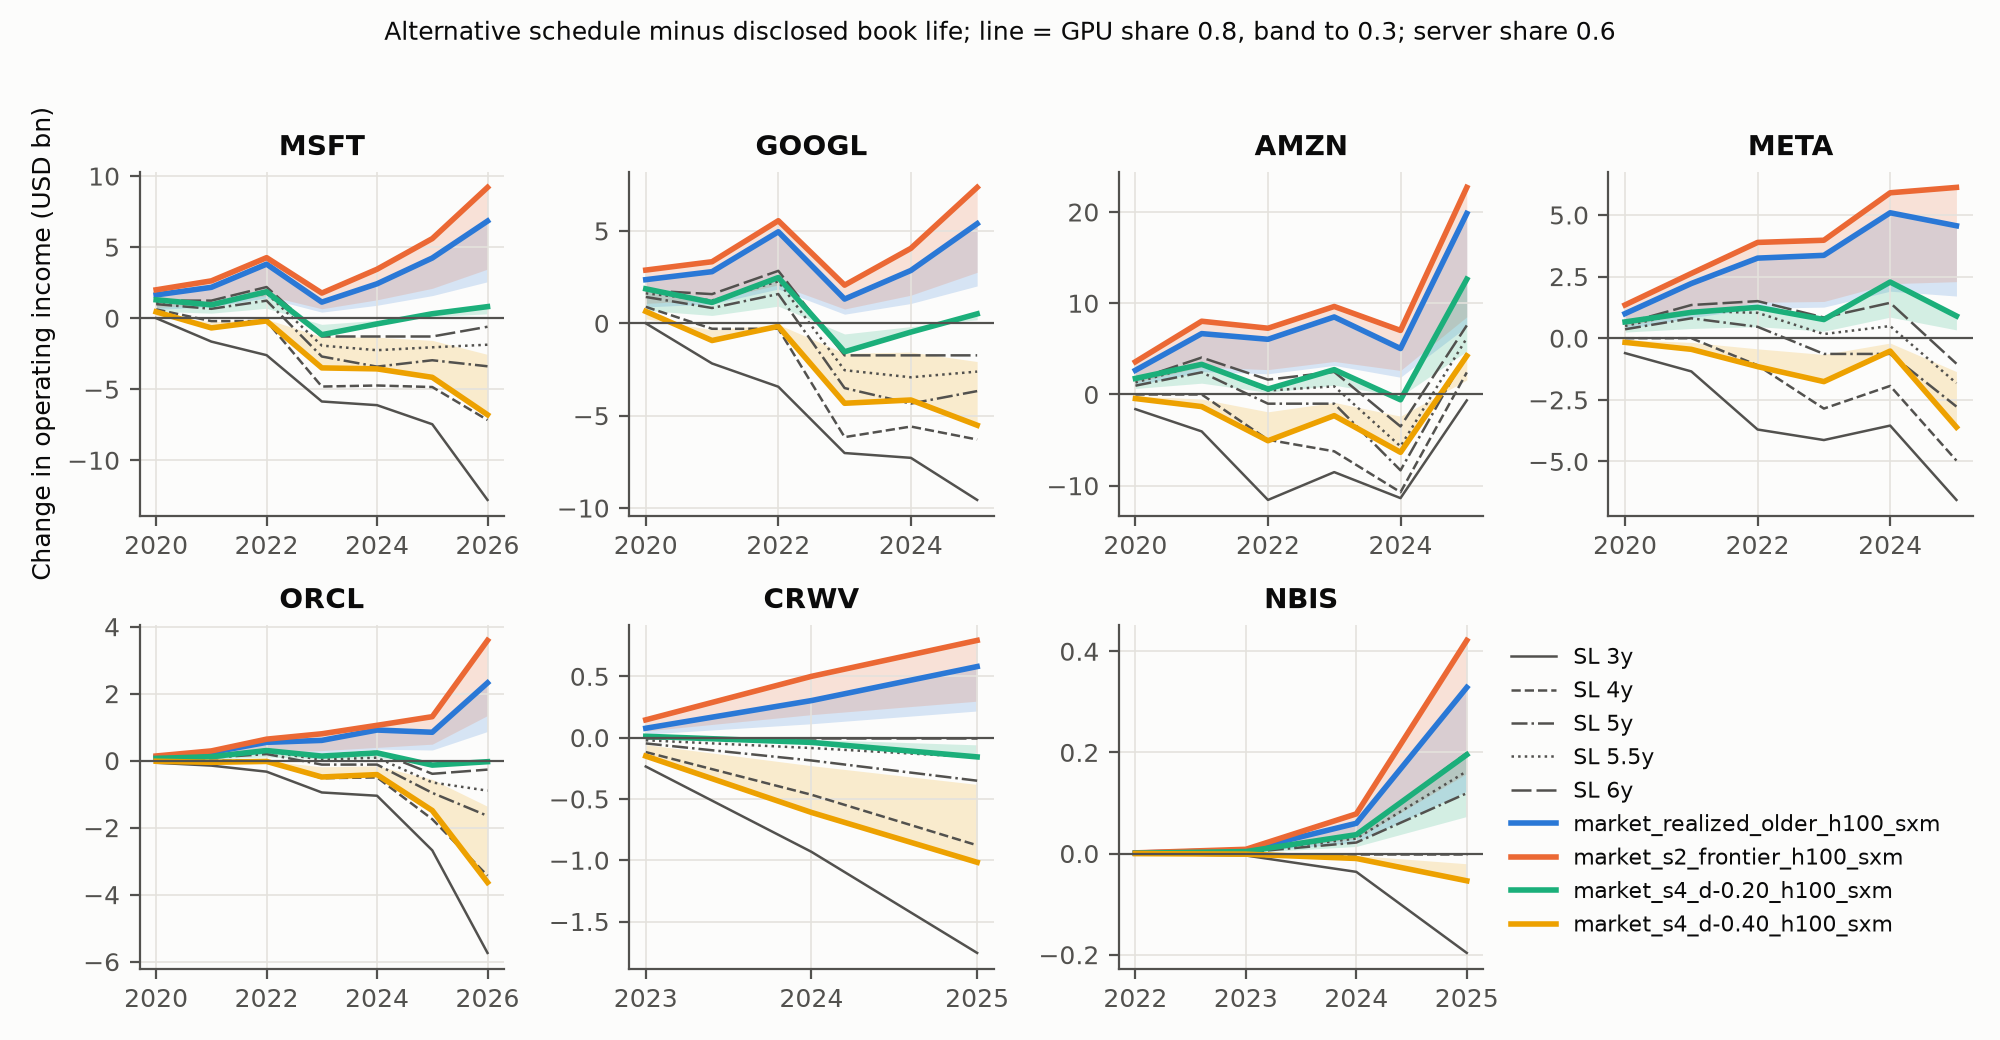
\includegraphics[width=0.85\textwidth]{p7_restatement.png}
\caption{Change in operating income by firm and schedule across the GPU-share grid.}
\label{fig:restate}
\end{figure}

\ajcheck{The sign of the restatement depends on the rent path, not on the method. Posted rents,
read through the realized paths, imply that book lives are, if anything, conservative. Only an
assumption of steep age-driven decline, which the rent data do not establish, produces the large
earnings overstatements discussed in the public debate.} The restatement inherits the limits of
the asset base: cash capital expenditure excludes finance-lease additions, which are material for
Amazon and Microsoft, and the server and GPU shares are assumptions shown as a grid.
}{\emph{Phase 7
restatement in progress.}}

\section{Robustness and limitations}
\label{sec:robust}

\paragraph{Contract type and sub-period.} Table~\ref{tab:h3h4} repeats the strategies by contract
type (H3) and sub-period (H4). The contract split is the important one (Section~\ref{sec:review}).
The sub-period split cannot test H4 as intended: 2026 alone covers under a year of each chip's
life, and before 2023 only three chips are on sale, too few clusters to report.

\begin{table}[htbp]
\centering
\caption{Age profile by contract type and sub-period}
\label{tab:h3h4}
\begin{adjustbox}{max width=\textwidth}
% Generated by gel.viz.hedonic_figures from p5_summary.csv. Do not edit.
% Rates in log points per year; early - late = rate(0-2) - rate(2-4); H1 predicts < 0.
\begin{tabular}{llccc}
\hline
Sample & Strategy & rate, yrs 0--2 & rate, yrs 2--4 & early $-$ late (H1: $<0$) \\
\hline
On demand & 1a quality index (TFLOP/s) & $-$0.07 [$-$0.47, 0.34] & 0.10 [$-$0.16, 0.37] & $-$0.17 [$-$0.70, 0.37] \\
On demand & 2 frontier-relative & $-$0.21 [$-$0.48, 0.07] & $-$0.09 [$-$0.36, 0.17] & $-$0.12 [$-$0.33, 0.08] \\
On demand & 4 shape only & -- & -- & $-$0.13 [$-$0.40, 0.13] \\
Reserved, 1 year & 1a quality index (TFLOP/s) & 0.81 [$-$0.54, 2.19] & 0.18 [$-$0.08, 0.45] & 0.63 [$-$0.78, 2.03] \\
Reserved, 1 year & 2 frontier-relative & 0.08 [$-$0.18, 0.34] & $-$0.06 [$-$0.23, 0.11] & 0.14 [$-$0.23, 0.50] \\
Reserved, 1 year & 4 shape only & -- & -- & 0.76 [$-$1.15, 2.66] \\
Reserved, 3 years & 1a quality index (TFLOP/s) & 0.19 [$-$0.07, 0.45] & 0.10 [$-$0.18, 0.37] & 0.09 [$-$0.05, 0.24] \\
Reserved, 3 years & 2 frontier-relative & $-$0.03 [$-$0.07, 0.01] & $-$0.12 [$-$0.28, 0.04] & 0.09 [$-$0.13, 0.31] \\
Reserved, 3 years & 4 shape only & -- & -- & $-$0.20 [$-$0.80, 0.38] \\
Spot & 1a quality index (TFLOP/s) & 0.46 [0.11, 0.81] & $-$0.19 [$-$0.32, $-$0.04] & 0.65 [0.19, 1.10] \\
Spot & 2 frontier-relative & 0.50 [0.18, 0.83] & $-$0.26 [$-$0.42, $-$0.09] & 0.76 [0.26, 1.26] \\
Spot & 4 shape only & -- & -- & 0.87 [0.34, 1.41] \\
Without Google, July 2026 & 1a quality index (TFLOP/s) & 0.28 [$-$0.21, 0.76] & $-$0.03 [$-$0.24, 0.18] & 0.31 [$-$0.50, 1.09] \\
Without Google, July 2026 & 2 frontier-relative & 0.11 [$-$0.12, 0.35] & $-$0.15 [$-$0.39, 0.10] & 0.26 [0.05, 0.47] \\
Without Google, July 2026 & 4 shape only & -- & -- & 0.47 [0.36, 0.57] \\
2023--2025 & 1a quality index (TFLOP/s) & 0.26 [$-$0.11, 0.63] & $-$0.27 [$-$0.43, $-$0.12] & 0.54 [0.19, 0.88] \\
2023--2025 & 2 frontier-relative & 0.11 [$-$0.09, 0.32]$^\dagger$ & $-$0.37 [$-$1.62, 0.86]$^\dagger$ & 0.48 [0.34, 0.63] \\
2023--2025 & 4 shape only & -- & -- & 0.48 [0.28, 0.68] \\
2026 & 1a quality index (TFLOP/s) & $-$0.36 [$-$53.25, 53.09] & $-$0.09 [$-$0.29, 0.12] & $-$0.27 [$-$52.97, 52.98] \\
2026 & 2 frontier-relative & $-$6.60 [$-$47.69, 35.77]$^\dagger$ & 0.82 [$-$2.86, 4.12]$^\dagger$ & $-$7.42 [$-$44.76, 30.91] \\
2026 & 4 shape only & -- & -- & $-$0.61 [$-$11.87, 10.71] \\
Provider-chip-months weighted equally & 1a quality index (TFLOP/s) & 0.21 [$-$0.21, 0.62] & $-$0.03 [$-$0.18, 0.11] & 0.24 [$-$0.15, 0.64] \\
Provider-chip-months weighted equally & 2 frontier-relative & 0.10 [$-$0.22, 0.43] & $-$0.08 [$-$0.17, 0.01] & 0.19 [$-$0.11, 0.47] \\
Provider-chip-months weighted equally & 4 shape only & -- & -- & 0.29 [0.07, 0.50] \\
\hline
\end{tabular}
% dagger: within-chip age span under 4 years with chip effects (extrapolated).

\end{adjustbox}
\par\smallskip\footnotesize As Table~\ref{tab:strategies}. $\dagger$: within-chip age span under
four years with chip effects (extrapolated). Sub-samples with fewer than six chips are not reported.
\end{table}

\paragraph{Weighting and composition.} Google Cloud is \nGoogleShare{} of the estimation sample.
Weighting each provider equally lowers the pooled shape to \nShapeEqualProv, and dropping Google
leaves \nShapeNoGoogle. Strategy 1's early-years rate depends on the H200: dropping it moves the
rate from \nOneARateEarly{} to \nOneARateEarlyNoHTwoHundred.

\paragraph{Posted versus transacted prices.} The panel is posted prices, overwhelmingly hyperscaler
list prices, and \nListUnchanged{} of on-demand and reserved month-to-month transitions are
unchanged. Large buyers pay negotiated prices that are not observed. \ajcheck{The results are
therefore about the posted-price market; a transacted-price panel, such as the marketplace data of
\citet{huang2026gpu}, would be the natural complement.}

\paragraph{Age zero.} Age is measured from Epoch's release month, which precedes the first cloud
listing by several months for some chips. The event study's sensitivity to that dating is reported
in Section~\ref{sec:events}.

\paragraph{Operating cost.} Hosting, network and staff costs are excluded for lack of a sourced
figure, so values are upper bounds and $T^*$ is biased upward.

\section{Conclusion}
\label{sec:conclusion}

Published estimates of accelerator depreciation disagree because they read different prices
through different assumptions. In a panel of posted rents for seven NVIDIA chips, realized
rents fall slowly; the shape of the age profile flips between spot and list prices; and with valid
few-cluster inference no identification strategy pins down the rate or the shape. Rents stay far
above operating cost for the whole observed life, so the economic life that matters for book
depreciation is decided by obsolescence in power-constrained data centers, not by rents reaching
operating cost.

\ajcheck{For accounting, the implication is narrower than either side of the public debate. Five-
or six-year straight-line lives are not contradicted by posted rents, whose value curves decline
more slowly than straight-line. They look long only if one believes that power-constrained
operators retire chips when a better chip arrives, which is what the retirement model and the
largest operators' own behavior suggest; even then the model's median retirement age of
\nPThreeMedian{} years has a P10--P90 range of \nPThreePTen--\nPThreePNinety{} years that contains
those lives. The firm-level effect of that choice is reported in
Section~\ref{sec:accounting}.}

The panel, code and identification range are public, so each of these choices can be revisited as
longer price histories for the Hopper and Blackwell generations accumulate.


\bibliographystyle{plainnat}
\bibliography{references}

\appendix
\section{Data and code availability}
\label{app:replication}

The replication package rebuilds every table and figure, and this paper, from the archived raw
files with one command (\texttt{make all}). Each raw file has a sidecar recording its source URL,
retrieval time and HTTP status. Prices from providers whose terms do not permit redistribution are
released as derived monthly aggregates; the SkyPilot catalog history and archived pages are
re-fetched by a script with checksums rather than redistributed. Methodological choices are logged
with dates and alternatives in \texttt{docs/decisions.md}, and every assumption with its value and
source in \texttt{docs/assumptions.md}.

\section{Adversarial review}
\label{app:review}

Before the results were written up, a reviewer with access only to the code, the result tables
and the identification section of the research proposal was asked for the weakest identifying
assumption and the most likely referee objection. Its fifteen points, the checks they led to and
the responses are in \texttt{docs/review\_01.md} and \texttt{docs/review\_01\_checks.md}; the
checks are in \texttt{gel.models.review\_checks} and Section~\ref{sec:review}.

\section{Statements}
\label{app:statements}

\paragraph{Use of AI tools.} This study was carried out with Claude, a language model made by
Anthropic, running in Claude Code. Under the author's direction, Claude wrote the collectors,
parsers and estimation code, ran the analyses, verified the references against their sources,
produced the figures and tables, and drafted the text of this paper; a separate instance with no
access to the author's notes wrote the adversarial review in Appendix~\ref{app:review}. The author
set the research questions and hypotheses, made or approved the methodological decisions logged
in the replication package, and takes responsibility for the content. No number in the paper is
typed by hand: each is generated by the replication package's code from archived data.

\paragraph{Declaration of interests.} None to declare.

\paragraph{Funding.} This research received no external funding.

\paragraph{Licences.} Code is released under the MIT licence; the text and the released dataset
under CC BY 4.0. Third-party data keep their sources' terms (Appendix~\ref{app:replication}).


\end{document}
